 % The main file for CAMP reports
 % Don't put any content in here. 
 % Don't even include content files by using \input or \inlcude. 
 % Put your content to TEXT.TEX or include it there using \input.
 % Uses:
 %		SETTINGS.TEX	contains the settings for this document
 %		COMMANDS.TEX	contains commands which can be used while writing
 %		INFO.TEX			contains the author, title and so on for the cover
 %		COVER.TEX			formats\documentclass[10pt]{?} the front cover of the document
 %		ABSTRACT.TEX	contains the abstract to be included (if needed)
 %		TEXT.TEX			contains the actual content of the document
 %		BIB.BIB				containt the BibTeX entries for the document
 
 
%% Draft document mode
%% Final document
\documentclass[11pt,a4paper,bibtotoc,idxtotoc,headsepline,footsepline,footexclude,BCOR12mm,DIV13]{scrbook}


%\documentclass[11pt,a4paper,bibtotoc,idxtotoc,headsepline,footsepline,footexclude,BCOR20mm,DIV10]{scrbook}

% KOMA-Optionen:
%  bibtotoc: include bibliography in table of contents
%  idxtotoc: include index in table of contents
%  headsepline: use horizontalline under heading
%  BCOR: binding correcion (Bindungskorrektur) (e.g.: BCOR5mm)
%  DIV: Number of sheet sections (used for layout) (e.g.: DIV12) 


% include title and author information for the cover
% Set here the title, authors and other stuff to be used for the cover
% This file is used by MAIN.TEX

% set title, authors and stuff for the cover
\def\doctype{Master's Thesis in Informatics}
\def\title{Materialized views with Apache Spark}
\def\titleGer{Materialisierte views mit Apache Spark}
\def\author{Saroj Gautam}
\def\date{August 15th, 2016}

% text to appear in the footer
\def\footertext{}

% include settings
% Included by MAIN.TEX
% Defines the settings for the CAMP report document

\renewcommand{\sectfont}{\normalfont \bfseries}        % Schriftart der Kopfzeile

% manipulate footer
\usepackage{scrpage2}
\pagestyle{scrheadings}
\ifoot[\footertext]{\footertext} % \footertext set in INFO.TEX
%\setkomafont{pagehead}{\normalfont\rmfamily}
\setkomafont{pagenumber}{\normalfont\rmfamily}

%% allow sophisticated control structures
\usepackage{ifthen}

% use Palatino as default font
\usepackage{palatino}

% enable special PostScript fonts
\usepackage{pifont}

% make thumbnails
\usepackage{thumbpdf}

%to use the subfigures
%\usepackage{subfigure}
\usepackage{caption}
\usepackage{subcaption}


\usepackage{colortbl}


%% show program code\ldots
%\usepackage{verbatim}
%\usepackage{program}

\usepackage{listings}


%% enable TUM symbols on title page
\usepackage{styles/tumlogo}


\usepackage{multirow}

%% use colors
\usepackage{color}

%% make fancy math
\usepackage{amsmath}
\usepackage{amsfonts}
\usepackage{amssymb}
\usepackage{textcomp}
\usepackage{yhmath} % f�r die adots 
%% mark text as preliminary
%\usepackage[draft,german,scrtime]{prelim2e}

%% create an index
\usepackage{makeidx}

% for the program environment
\usepackage{float}

%% load german babel package for german abstract
%\usepackage[german,american]{babel}
\usepackage[german,english]{babel}
\selectlanguage{english}

% use german characters as well
\usepackage[latin1]{inputenc}       % allow Latin1 characters

% use initals dropped caps - doesn't work with PDF
%\usepackage{dropping}

% Load the package
\usepackage{glossaries}

\usepackage{styles/shortoverview}
%----------------------------------------------------
%      Graphics and Hyperlinks
%----------------------------------------------------

%% check for pdfTeX
\ifx\pdftexversion\undefined
 %% use PostScript graphics
 \usepackage[dvips]{graphicx}
 \DeclareGraphicsExtensions{.eps,.epsi}
 \graphicspath{{figures/}{figures/review}} 
 %% allow rotations
 \usepackage{rotating}
 %% mark pages as draft copies
 %\usepackage[english,all,light]{draftcopy}
 %% use hypertex version of hyperref
 \usepackage[hypertex,hyperindex=false,colorlinks=false]{hyperref}
\else %% reduce output size \pdfcompresslevel=9
 %% declare pdfinfo
 %\pdfinfo { 
 %  /Title (my title) 
 %  /Creator (pdfLaTeX) 
 %  /Author (my name) 
 %  /Subject (my subject	) 
 %  /Keywords (my keywords)
 %}
 %% use pdf or jpg graphics
 \usepackage[pdftex]{graphicx}
 \DeclareGraphicsExtensions{.jpg,.JPG,.png,.pdf,.eps}
 \graphicspath{{figures/}} 
 
 %% Load float package, for enabling floating extensions
 \usepackage{float}
 
 %% allow rotations
 \usepackage{rotating}
 %% use pdftex version of hyperref
 \usepackage[pdftex,colorlinks=true,linkcolor=black,citecolor=black,%
 anchorcolor=black,urlcolor=black,bookmarks=true,%
 bookmarksopen=true,bookmarksopenlevel=0,plainpages=false%
 bookmarksnumbered=true,hyperindex=false,pdfstartview=%
 ]{hyperref}
%
%\usepackage[pdftex,colorlinks=false,linkcolor=red,citecolor=red,%
% anchorcolor=red,urlcolor=red,bookmarks=true,%
% bookmarksopen=true,bookmarksopenlevel=0,plainpages=false%
% bookmarksnumbered=true,hyperindex=false,pdfstartview=%
% ]{hyperref}
\fi




%% Fancy chapters
%\usepackage[Lenny]{fncychap}
%\usepackage[Glenn]{fncychap}
%\usepackage[Bjarne]{fncychap}

%\usepackage[avantgarde]{quotchap}

% set the bibliography style
%\bibliographystyle{styles/bauermaNum}
%\bibliographystyle{alpha}
\bibliographystyle{plain}

% include commands
% Commands to be used within the TUM report document
% Included by MAIN.TEX
% Please include your own cool commands here. 
% Be only sure to comment it sufficiently so others can use it.

%-------------------------------------------------------------
%                      Own Commands
%-------------------------------------------------------------


%-------------------------------------------------------------
% math stuff -------------------------------------------------

% nice R, N, C
\newcommand{\nat}{\mathbb{N}}
\newcommand{\real}{\mathbb{R}}
\newcommand{\compl}{\mathbb{C}}



% norm
\newcommand{\norm}[1]{\left\| #1 \right\|}

% un demi
\newcommand{\half}{\frac{1}{2}}

% parantheses
\newcommand{\parenth}[1]{ \left( #1 \right) }
\newcommand{\bracket}[1]{ \left[ #1 \right] }
\newcommand{\accolade}[1]{ \left\{ #1 \right\} }
%\newcommand{\angle}[1]{ \left\langle  #1 \right\rangle }

% partial derivative: %#1 function, #2 which variable
% simple / single line version
\newcommand{\pardevS}[2]{ \delta_{#1} f(#2) }
% fraction version
\newcommand{\pardevF}[2]{ \frac{\partial #1}{\partial #2} }

% render vectors: 3 and 4 dimensional
\newcommand{\veciii}[3]{\left[ \begin{array}[h]{c} #1 \\ #2 \\ #3	\end{array} \right]}
\newcommand{\veciv}[4]{\left[ \begin{array}[h]{c} #1 \\ #2 \\ #3 \\ #4	\end{array} \right]}

% render matrices: 3  dimensional (arguments in row first order)
\newcommand{\matiii}[9]{\left[ \begin{array}[h]{ccc} #1 & #2 & #3 \\ #4 & #5 & #6 \\ #7 & #8 & #9	\end{array} \right]}
%DOESN'T WORK,DON'T KNOW WHY \newcommand{\mativ}[16]{\left[ \begin{array}[h]{cccc} #1 & #2 & #3 & #4 \\ #5 & #6 & #7 & #8 \\ #9 & #10 & #11 & #12 \\ #13 & #14 & #15 & #16 \end{array} \right]}


%-------------------------------------------------------------
%-------------------------------------------------------------


%-------------------------------------------------------------
% some abreviations ------------------------------------------
\newcommand{\Reg}{$^{\textregistered}$}
\newcommand{\reg}{$^{\textregistered}$ }
\newcommand{\Tm}{\texttrademark}
\newcommand{\tm}{\texttrademark~}
\newcommand {\bsl} {$\backslash$}

%-------------------------------------------------------------
%-------------------------------------------------------------


%-------------------------------------------------------------
% formating --------------------------------------------------

% Theorem & Co environments and counters
\newtheorem{theorem}{Theorem}[chapter]
\newtheorem{lemma}[theorem]{Lemma}
\newtheorem{corollary}[theorem]{Corollary}
\newtheorem{remark}[theorem]{Remark}
\newtheorem{definition}[theorem]{Definition}
\newtheorem{equat}[theorem]{Equation}
\newtheorem{example}[theorem]{Example}
\newtheorem{algorithm}[theorem]{Algorithm}

% inserting figures
\newcommand{\insertfigure}[4]{ % Filename, Caption, Label, Width percent of textwidth
	\begin{figure}[htbp]
		\begin{center}
			\includegraphics[width=#4\textwidth]{#1}
		\end{center}
		\vspace{-0.4cm}
		\caption{#2}
		\label{#3}
	\end{figure}
}




% referecing figures

\newcommand{\refFigure}[1]{ %label
	figure \ref{#1}
}
\newcommand{\refChapter}[1]{ %label
	chapter \ref{#1}
}

\newcommand{\refSection}[1]{ %label
	section \ref{#1}
}

\newcommand{\refParagraph}[1]{ %label
	paragraph \ref{#1}
}

\newcommand{\refEquation}[1]{ %label
	equation \ref{#1}
}

\newcommand{\refTable}[1]{ %label
	table \ref{#1}
}




\newcommand{\rigidTransform}[2]
{
	${}^{#2}\!\mathbf{H}_{#1}$
}

%code, in typewriter
\newcommand{\code}[1]
 {\texttt{#1}}

% comment that appears on the border - very practical !!!
\newcommand{\comment}[1]{\marginpar{\raggedright \noindent \footnotesize {\sl #1} }}

% page clearing
\newcommand{\clearemptydoublepage}{%
  \ifthenelse{\boolean{@twoside}}{\newpage{\pagestyle{empty}\cleardoublepage}}%
  {\clearpage}}


%-------------------------------------------------------------
%-------------------------------------------------------------


\newcommand{\etAl}{\emph{et al.}\mbox{ }}


%\makeindex
	%% inter line spacing
%\linespread{1.0}

\makeglossary

\begin{document}

	\frontmatter
	
	
	% The front cover for the TUM report document.
% Included by MAIN.TEX


%--------------------------------------------------
% The Front Cover
%--------------------------------------------------

% The front cover for the TUM document.
% Included by MAIN.TEX


%--------------------------------------------------
% The Front Cover
%--------------------------------------------------

% correct BCOR - undo at the end !!!
\def\bcorcor{0.15cm}
\addtolength{\hoffset}{\bcorcor}

\thispagestyle{empty}

 \vspace{4cm}
\begin{center}
	       \oTUM{4cm}
	   
	   \vspace{5mm}     
	   \huge FAKULT{\"A}T F{\"U}R INFORMATIK\\ 
	   \vspace{0.5cm}
	 \large DER TECHNISCHEN UNIVERSIT{\"A}T M{\"U}NCHEN\\
    \vspace{1mm}
        
	\end{center}
		

\vspace{15mm}
\begin{center}

   {\Large \doctype}

  \vspace{20mm}
  
  {\huge\bf \title}\\%[3ex]
  
  
  \vspace{15mm}
  
  
  {\LARGE  \author}
  
  \vspace{10mm}
  
  \begin{figure}[h!]
  \centering
   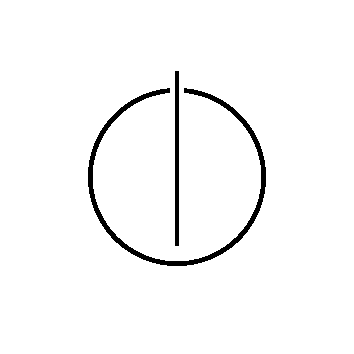
\includegraphics[width=4cm]{styles/informat.png}
  \end{figure}
  
  \end{center}
%	\clearemptydoublepage
	
	%% The titlepage for the CAMP report document.
% Included by MAIN.TEX


%--------------------------------------------------
% The title page
%--------------------------------------------------

% correct BCOR - undo at the end !!!
\def\bcorcor{0.15cm}
\addtolength{\hoffset}{\bcorcor}

\thispagestyle{empty}

 \vspace{10mm}
\begin{center}
	       \oTUM{4cm}
	   
	   \vspace{5mm}     
	   \huge FAKULT{\"A}T F{\"U}R INFORMATIK\\ 
	   \vspace{0.5cm}
	 \large DER TECHNISCHEN UNIVERSIT{\"A}T M{\"U}NCHEN\\
        
	\end{center}
		

\vspace{10mm}
\begin{center}

   {\Large \doctype}

  \vspace{10mm}
  
  {\LARGE \title}\\
  
  
  \vspace{10mm}
  
  
  {\LARGE  \titleGer}\\
  
  
  \vspace{10mm}

    %\hfill
    \begin{tabular}{ll}
	   \Large Author:     & \Large \author \\[2mm]
	   \Large Supervisor:    & \Large Prof. Dr. Hans-Arno Jacobsen \\[2mm]				
	   \Large Advisor:	& \Large M. Sc. Jan Adler\\[2mm]
	   \Large Date:       & \Large August 15, 2016
	 \end{tabular}
	 
	 \vspace{5mm}
	 
	 \begin{figure}[h!]
  \centering
   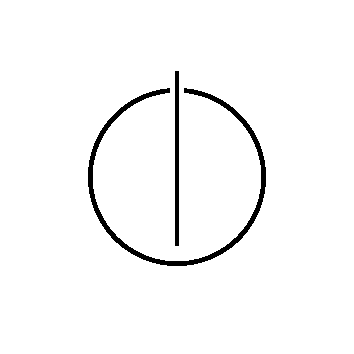
\includegraphics[width=4cm]{styles/informat.png}
  \end{figure}
   

\end{center}

% undo BCOR correction
\addtolength{\hoffset}{\bcorcor}
	
	
%	\input{components/cover_maschmeyer}
	\clearemptydoublepage
	
	% The titlepage for the CAMP report document.
% Included by MAIN.TEX


%--------------------------------------------------
% The title page
%--------------------------------------------------

% correct BCOR - undo at the end !!!
\def\bcorcor{0.15cm}
\addtolength{\hoffset}{\bcorcor}

\thispagestyle{empty}

 \vspace{10mm}
\begin{center}
	       \oTUM{4cm}
	   
	   \vspace{5mm}     
	   \huge FAKULT{\"A}T F{\"U}R INFORMATIK\\ 
	   \vspace{0.5cm}
	 \large DER TECHNISCHEN UNIVERSIT{\"A}T M{\"U}NCHEN\\
        
	\end{center}
		

\vspace{10mm}
\begin{center}

   {\Large \doctype}

  \vspace{10mm}
  
  {\LARGE \title}\\
  
  
  \vspace{10mm}
  
  
  {\LARGE  \titleGer}\\
  
  
  \vspace{10mm}

    %\hfill
    \begin{tabular}{ll}
	   \Large Author:     & \Large \author \\[2mm]
	   \Large Supervisor:    & \Large Prof. Dr. Hans-Arno Jacobsen \\[2mm]				
	   \Large Advisor:	& \Large M. Sc. Jan Adler\\[2mm]
	   \Large Date:       & \Large August 15, 2016
	 \end{tabular}
	 
	 \vspace{5mm}
	 
	 \begin{figure}[h!]
  \centering
   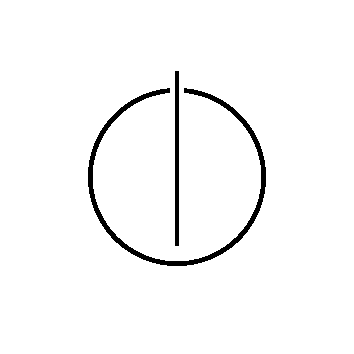
\includegraphics[width=4cm]{styles/informat.png}
  \end{figure}
   

\end{center}

% undo BCOR correction
\addtolength{\hoffset}{\bcorcor}
	
	
	\clearemptydoublepage


\thispagestyle{empty}
\selectlanguage{english}
	\vspace*{0.8\textheight}
	\noindent
	I assure the single handed composition of this master's thesis, only supported by declared resources.
	\newline
	\newline
	\newline
	\noindent
	M{\"u}nchen, August 15th, 2016 \hspace{5cm} \author
\selectlanguage{english}
\newpage
	
	\clearemptydoublepage
\phantomsection
\addcontentsline{toc}{chapter}{Acknowledgements}	


%\chapter*{Acknowledgements}

\vspace*{2cm}

\begin{center}
{\Large \bf Acknowledgments}
\end{center}

\vspace{1cm}

I would first like to thank my advisor Jan Adler for providing me the opportunity to work on an interesting topic and supervising me throughout the research. 
\newline

I thank Prof. Dr. Hans-Arno Jacobsen for providing me an opportunity to write my thesis under the Chair of Distributed Systems. I thank my advisor for providing me valuable feedbacks and suggestion from the start to the end of the thesis.
\newline

I would like to thank my family for giving me the motivation and moral support. I would also like to thank my friends Suvash Sedhain and Niroj Sapkota for their constant support and motivation. And special thanks to my friends for creating a positive environment by cracking jokes and taking off the pressure during coffee breaks.

	
	% Abstract for the TUM report document
% Included by MAIN.TEX


\clearemptydoublepage
\phantomsection
\addcontentsline{toc}{chapter}{Abstract}	





\vspace*{2cm}
\begin{center}
{\Large \bf Abstract}
\end{center}
\vspace{1cm}

% In today's world where billions of people exchange information online, service providers like Facebook, Twitter, Whatsapp store and process tremendous amount of data. Those service providers need distributed scalable storage systems to store and process big volume of data. Even though data are stored in a distributed storage systems, still the huge size of data are bottleneck for performance optimization. Scanning tens of millions rows and few million columns each time are expensive in terms of execution time and processing power. $Materialized$ $Views$ solve this problem by precomputing expensive queries and storing result in a physical table or disk. One of the bottleneck for this approach is constantly maintaining consistency between base table and view table. We propose a $Incremental$ $View$ $Maintenance$ approach to maintain consistency between base table and view table.


In today's world, billions of people exchange information online. Service providers like Facebook, Twitter, Whatsapp store and process tremendous amount of data. Those service providers need distributed scalable storage systems to store and process a big volume of data. Even though data are stored in a distributed storage systems, still the huge size of data can be a bottleneck regarding performance optimization. Scanning tens of millions of rows and few million columns each time are expensive regarding execution time and processing power. $Materialized$ $Views$ solve this problem by pre-computing expensive queries and storing the result in a physical table or disk. One of the bottlenecks for this approach is constantly maintaining consistency between the base table and the view table. In this thesis, we propose a $Incremental$ $View$ $Maintenance$ approach to maintain consistency between the base table and the view table.

	\tableofcontents
  
 % \clearemptydoublepage

\phantomsection
\addcontentsline{toc}{chapter}{Outline of the Thesis}

\begin{center}
	\huge{Outline of the Thesis}
\end{center}




%--------------------------------------------------------------------
\section*{Part I: Introduction and Theory}

\noindent {\scshape Chapter 1: Introduction}  \vspace{1mm}

\noindent  This chapter presents an overview of the thesis and it purpose. Furthermore, it will discuss the sense of life in a very general approach.  \\

\noindent {\scshape Chapter 2: Theory}  \vspace{1mm}

\noindent  No thesis without theory.   \\

%--------------------------------------------------------------------
\section*{Part II: The Real Work}

\noindent {\scshape Chapter 3: Overview}  \vspace{1mm}

\noindent  This chapter presents the requirements for the process.

	\mainmatter
	
	



\chapter{Introduction}
\label{chap:introduction}

Whenever we see our friends posting pictures on Facebook or Instagram, we generally like them or comment on them. Whenever we feel like sharing our thoughts, we either update status on Facebook or just tweet about it. If we need some relevant information, we just google it. The amount of data generated in such a fashion has to be stored somewhere. Companies like Facebook stores 500 TB of data each day\cite{daniel:datastats}, including 2.7 billion likes and 300 million photos. As of 2012, Facebook already has 100 petabyte of photos\cite{daniel:datastats}. Google, on the other hand processes 3.5 billion request per day \cite{daniel:datastats}. In Early 2000s, where there were less data shared on social media, data were stored in a relational database. Relational database were designed in such a fashion to store small amount of data and maintain integrity between them\cite{matt:rdb}. The amount of information we share on social media is expected to grow from 4.4 zettabytes in 2013 to 44 zettabytes in 2020(1 zettabyte is 1 trillion gigabytes)\cite{matt:rdb}. The scaling in RDBMS depends on adding more powerful CPU's and memory, i.e. only the vertical scaling is possible which is rather expensive.  One of the advantages of big data storage system is that it can be scaled horizontally and is also useful for storing unstructured or semi structured data. 

HBase is an open source sortedMap Datastore from Apache Software Foundation which is used as a database to store huge volume of data. HBase supports horizontal scalability, i.e. parts of a table can be put on several machines. This way a table is broken down to multiple pieces, thus making computation really fast. But when we are talking about petabytes of data, scanning each part of table for a single user query is still considered to be expensive in terms of processing time. There are several techniques to reduce this effort, but we will be talking about $Materialized$ $Views$ approach. 


%In Chapter \ref{chap:background}, we analyse the fundamentals of views and view maintenance. In Chapter \ref{chap:relatedwork}, we present research, that is related to this thesis. In Chapter \ref{chap:analysis}, we define the requirements of the View Maintenance System and discuss possible alternatives.  In Chapter \ref{chap:architecture}, we align the architecture of the system and define its functionalities. In Chapter \ref{chap:viewconsistency}, we discuss threats to consistency and apply consistency techniques. In Chapter \ref{chap:loadbalancing}, we show how load balancing can be accomplished in the View Maintenance System. In Chapter \ref{chap:failuredetection}, we take counter measures to component failure. In Chapter \ref{chap:implementation}, we show challenges of the implementation. Finally, we evaluate and interpret the behaviour of the system in Chapter \ref{chap:evaluation}.\\%


\chapter{Background}
\label{chap:background}

In this chapter we will first discuss about the fundamentals of $Materialized$ $Views$ and $View$ $Types$. We will further explain about the technologies used widely in today's Distributed Storage Databases. 

\section{Materialized Views}

Materialized views are defined as the database object that stores the result of a query in a table or a disk. Materialized views are widely used for gaining performance advantage, i.e. to speed up query processing time over large datasets. The need for Materialized view addresses the problem of having to query large datasets that often needs joins and aggregations between multiple tables. These kind of queries are very expensive, in terms of execution time and processing power. Materialized views speeds up the query processing time by pre-computing joins and aggregations prior to execution and stores these results in a table or disk\cite{materializedview:oracle}. 

\section{View Maintenance}
Once the Materialized views are created, our query is redirected to Materialized View table rather than base table. Whenever there is an update in the base table, the Materialized View table also has to be updated accordingly. One of the solutions would be recomputing the whole Materialized View from the scratch or using the heuristic of inertia\cite{maintenance:materializedviews} approach i.e. incremental maintenance with respect to the base table.

\section{Incremental Maintenance of Materialized View}
"A view V is considered consistent with the database DB if the evaluation of the view specification S over the database yields the view instance (V = S(DB)). Therefore, when the database DB is updated to DB0 , we need to update the view V to V0 = S(DB0) in order to preserve its consistency"\cite{incrementalmaintenance:materializedviews}. 

Recomputing Materialized view from scratch every time there is an update on base table is expensive. The other approach is to update the part of Materialized view table with respect to the update in Base Table. Our target is to maintain consistency between Materialized views and base table whenever there is an update on the base table.


\subsection{Aggregation}
In Aggregation view type, the data of base table is merged on the basis of a particular key. In our implementation, we've implemented basic aggregation functions like sum, count, min and max. All these operations are carried out based on a particular key. So a unique key has sum, count, min and max operations. Whenever an update is triggered to update value for a particular key in the base table, in this case, count remains same and sum, min and max has to be recalculated. If a delete is triggered for a particular key in the base table, each of the aggregation functions has to be recalculated. 


\subsection{Join and Aggregation}
In Join and Aggregation case, we have at least two base tables. Joins being one of the complex structure itself, incremental view maintenance implementation involves a lot of complex cases. Here, to reduce complexity, we join two base tables on the basis of $key$ to form a new intermediate table. We group all the values of both base tables based on their keys. This way, for any update or delete trigger, the complexity of scanning whole base table is reduced to a single row. In our intermediate table, each of the base table is merged to a column family, join is applied and then result is stored in the view table. 

In the intermediate table, the unique keys from both the base tables act as the row key, both column families from base table are merged in the intermediate table. Now for a particular row key, the values are selected from base table and plotted in the intermediate table. Now join is applied between both column families of a particular row key, and sum of the join is inserted in the view table.  


\subsection{Join and Selection}
Join and Selection case is similar to the Join and Aggregation case, the only difference is instead of applying aggregation function, the join is applied for a particular row key and value is selected and inserted into the view table.


\section{HBase}
\label{sec:hbase}

HBase is an open source sortedMap Datastore from Apache Software Foundation. HBase is modeled after Google's BigTable framework. A basic table structure of HBase consists of Row Key, which is similar to the primary key in relational database table, Column Family and Column Qualifier.  

\begin{figure}
	\centering
	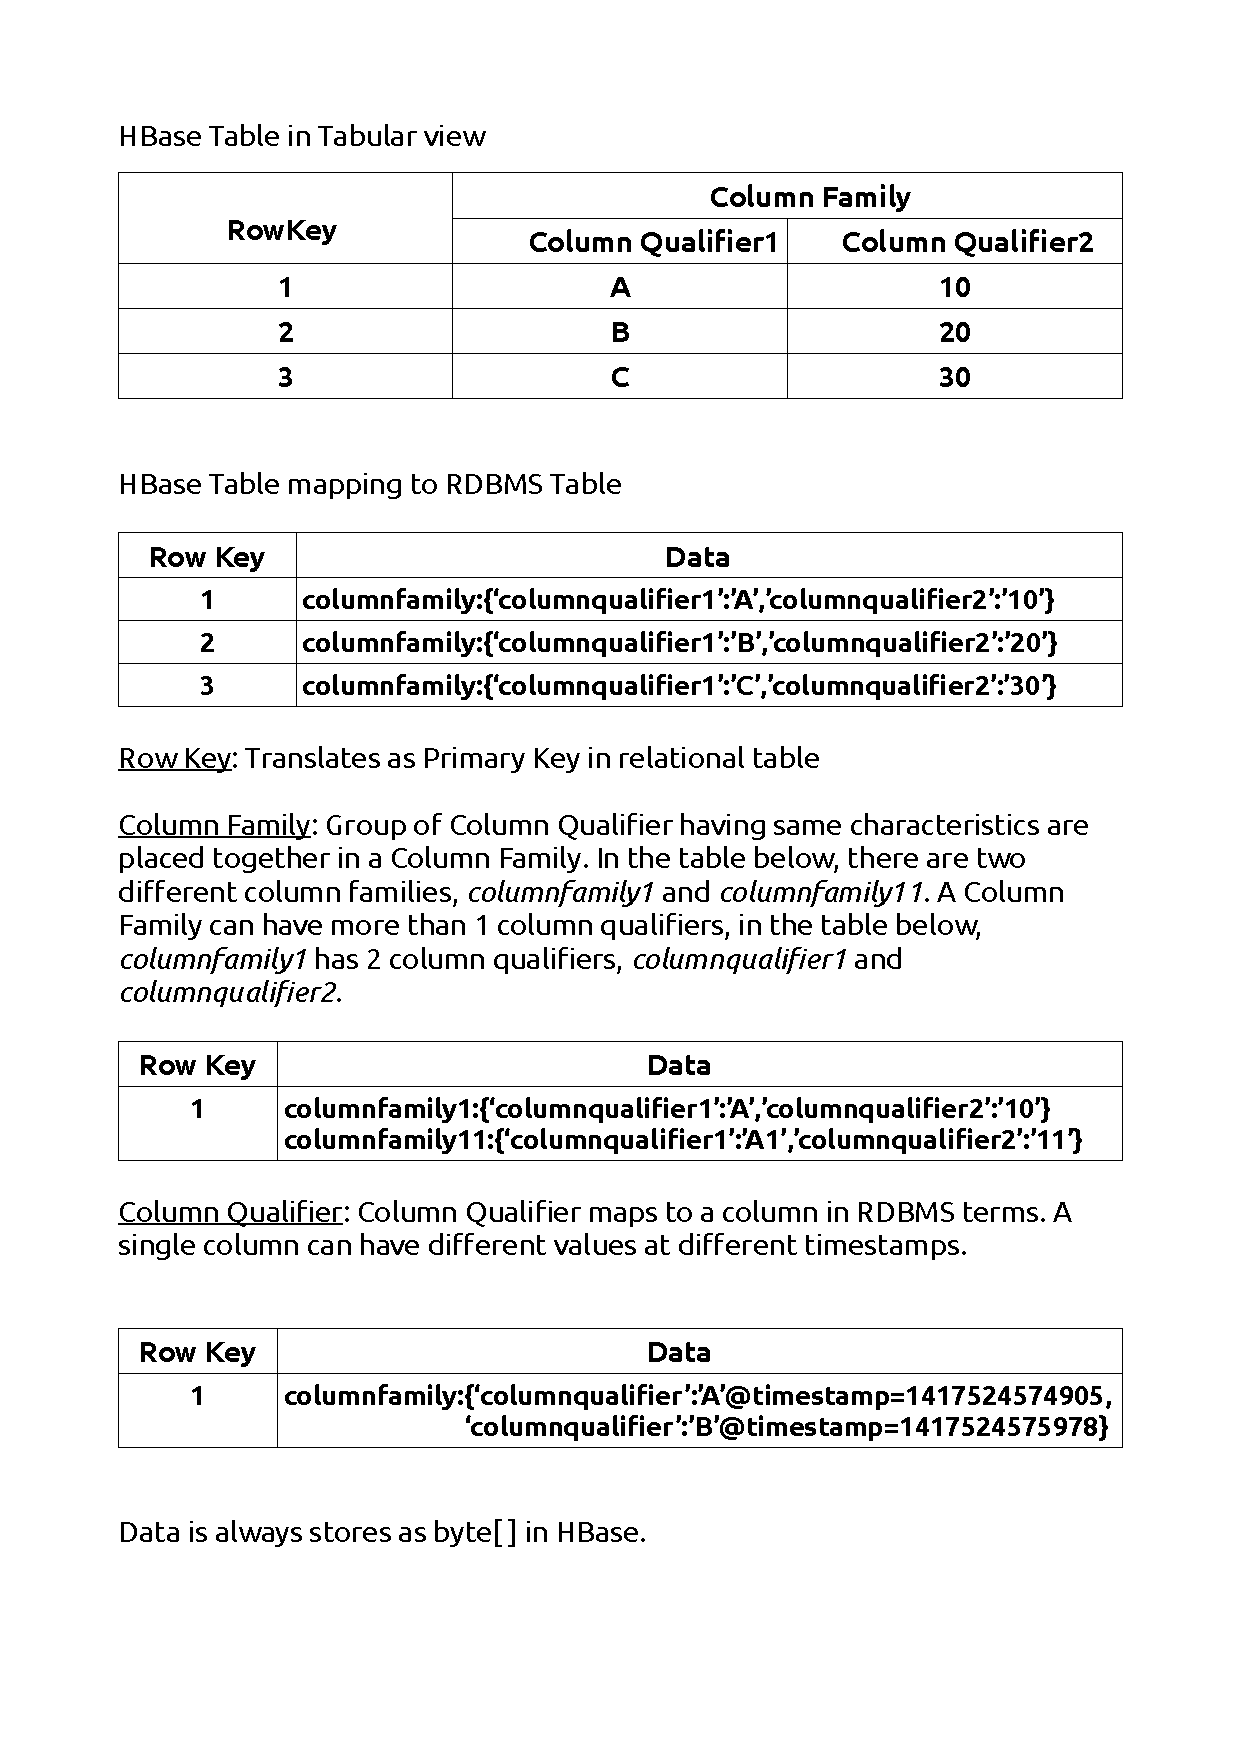
\includegraphics[width=\linewidth]{HBase}
	\caption{HBase Table}
	\label{fig:hbasetable}
\end{figure}



		% ---------------------------------------------------------------------------
		%
		% Appendix
		%
		% ---------------------------------------------------------------------------
		
		\part*{Appendix}
		\addcontentsline{toc}{part}{Appendix}
		
		\appendix %---------------------------------------
		
		%\chapter{Components}
%\section{Detailed Validation Results}
\label{chapter:Components}

\section{VM Master}


\textbf{Interface}

\begin{enumerate}
	\item Ingoing
	\begin{itemize}
		\item $viewManagerAdded$
		\item $viewManagerAssigned$
		\item $viewManagerRemoved$
		\item $viewManagerWithdrawn$
		\item $viewManagerReassigned$
		\item $regionServerAdded$
		\item $regionServerRemoved$
		\item $callLastCommitedUpdate$
	\end{itemize}
	\item Outgoing
	\begin{itemize}
		\item $createZookeperNode$
		\item $assignViewManager$
		\item $reassignViewManager$
		\item $withdrawViewManager$
		\item $removeViewManager$
		\item $replayWriteAheadLog$

	\end{itemize}
\end{enumerate}


\textbf{Subcomponents}

\begin{enumerate}
	\item $VM\:Master\:Controller$
	\item $Event\:Processor$
	\item $Load\:Balancer$
	\item $Recover\:Manager$
	\item $Component\:Controller$
\end{enumerate}
\newpage
\begin{figure}[h!] 
  \centering
    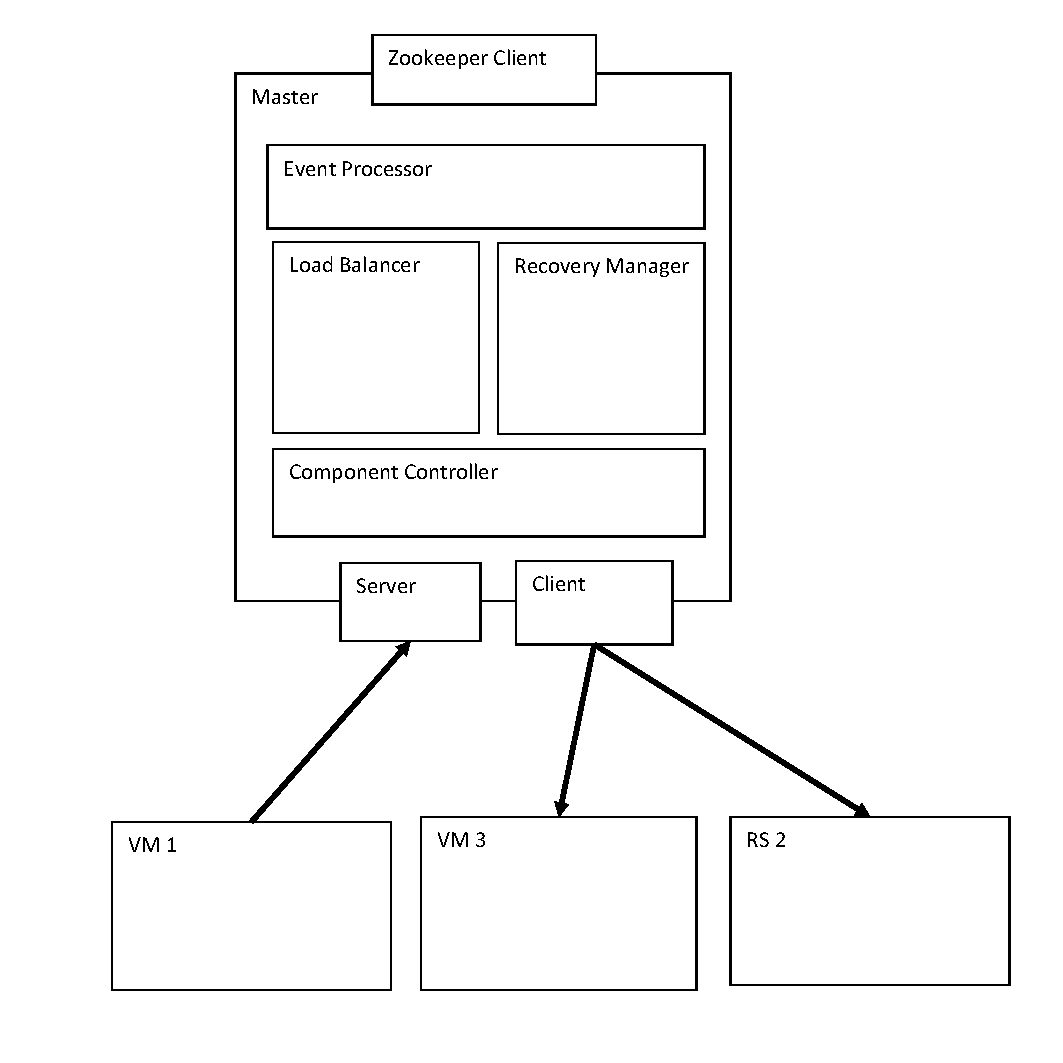
\includegraphics[scale=0.8]{figures/Master}
    \caption{Master}
    \label{fig:master}
\end{figure}

\newpage

\section{VM Region Server}

\textbf{Interface}

\begin{enumerate}
	\item Ingoing
	\begin{itemize}
		\item $put, get, delete$
		\item $assignViewManager$
		\item $withdrawViewManager$
		\item $replayWriteAheadLog$
		\item $statusReportViewManager$
	\end{itemize}
	\item Outgoing
	\begin{itemize}
		\item $createZookeeperNode$
		\item $sendUpdate$
		\item $sendStatusReport$
	\end{itemize}
\end{enumerate}


\textbf{Subcomponents}

\begin{enumerate}
	\item $HBase\:Region\:Server$
	\item $RS\:Controller$
	\item $Write\:Ahead\:Log$
	\item $WAL\:Reader$
	\item $Update\:Assigner$
	\item $Update\:Distributor$
\end{enumerate}

\newpage
\begin{figure}[h!]
  
  \centering
    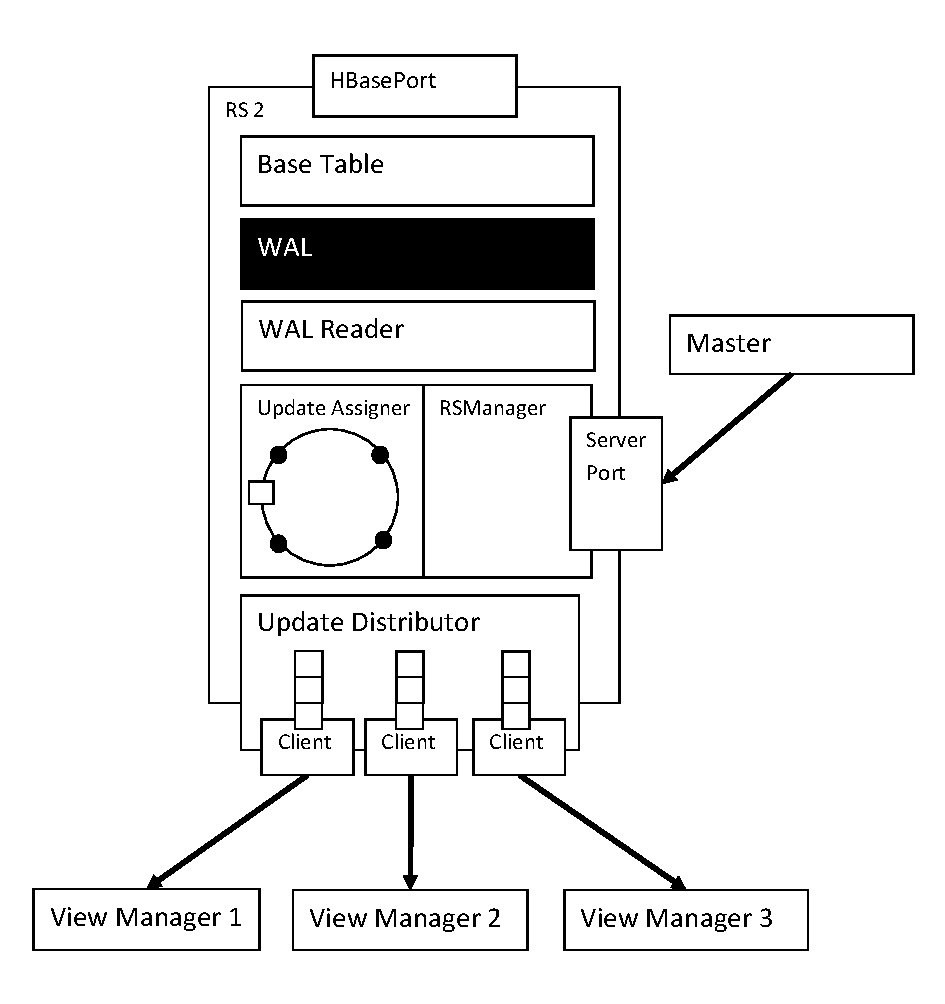
\includegraphics[scale=0.8]{figures/RegionServer}
    \caption{Region Server}
    \label{fig:regionserverAppendix}
\end{figure}
\newpage

\section{View Manager}



\textbf{Interface}

\begin{enumerate}
	\item Ingoing
	\begin{itemize}
		\item $receiveUpdate$
		\item $assignViewManager$
		\item $withdrawViewManager$
		\item $reassignViewManager$
		\item $removeViewManager$
		\item $callLastCommitedUpdate$
	\end{itemize}
	\item Outgoing
	\begin{itemize}
		\item $createZookeeperNode$
		\item $shutdownViewManager$
		\item $assignViewManager$
		\item $withdrawViewManager$
		\item $getViewDefinitions$
		\item $sendStatusReport$

	\end{itemize}
\end{enumerate}

\textbf{Subcomponents}

\begin{enumerate}
	\item $VM\:Controller$
	\item $Pre-Processor$
	\item $Processor$
	\item $Commit\:Log$
\end{enumerate}

\newpage

\begin{figure}[h!]
  
  \centering
    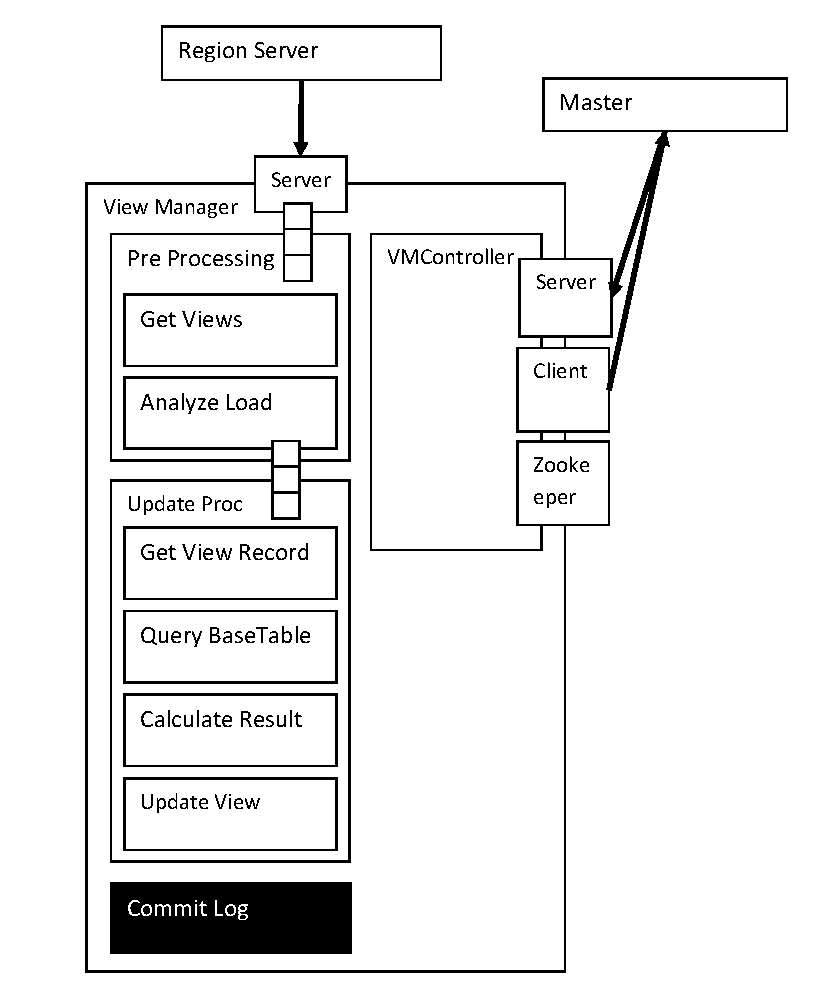
\includegraphics[width=\linewidth]{figures/ViewManager}
    \caption{View Manager}
    \label{fig:viewmanager}
\end{figure}
\newpage



\chapter{System Operations}
\label{chapter:Sytem Operations}


\section{Add View Manager}
\begin{figure}[h!]
  \centering
    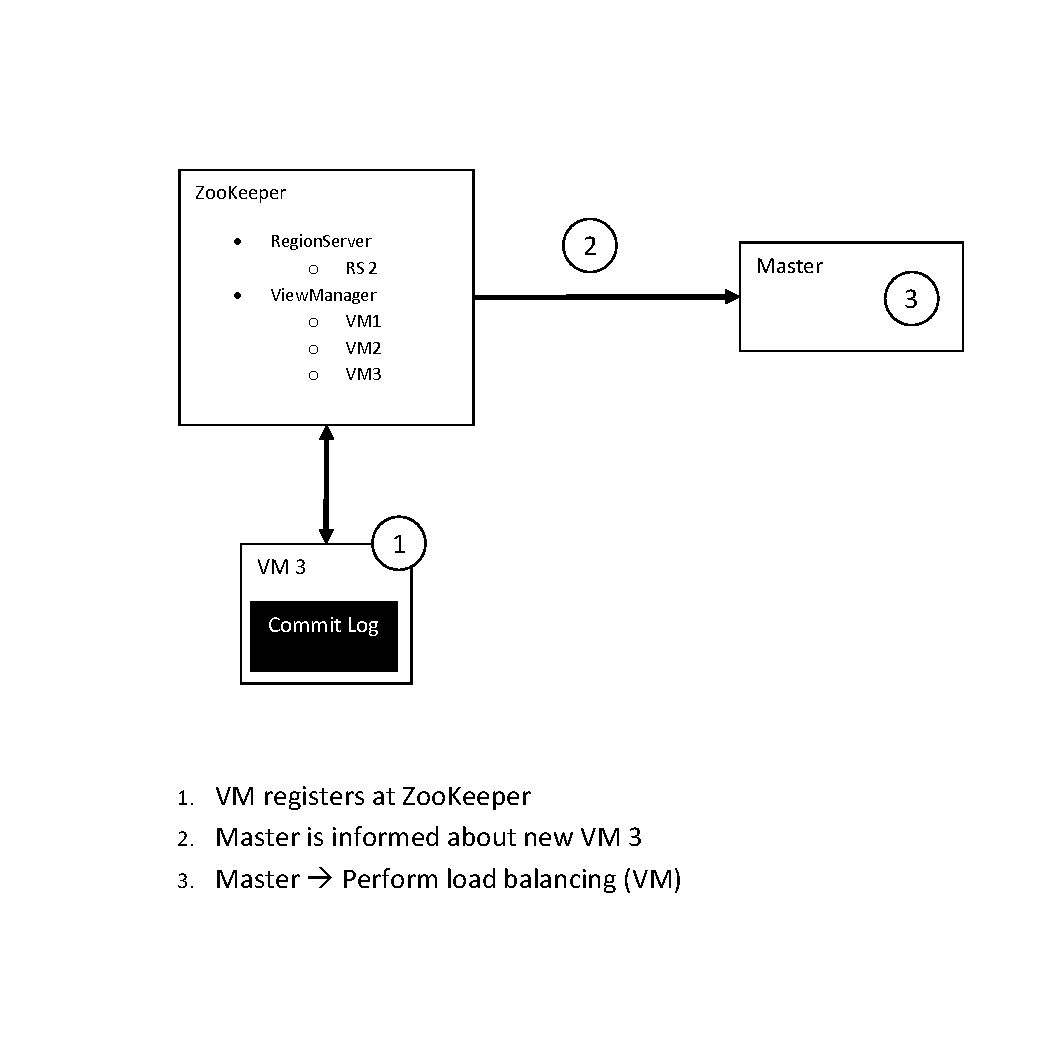
\includegraphics[scale=0.8]{figures/SO_AddViewManager}
    \caption{Add View Manager}
    \label{fig:addviewmanager}
\end{figure}
\newpage

\section{Assign View Manager}
\begin{figure}[h!]
  \centering
    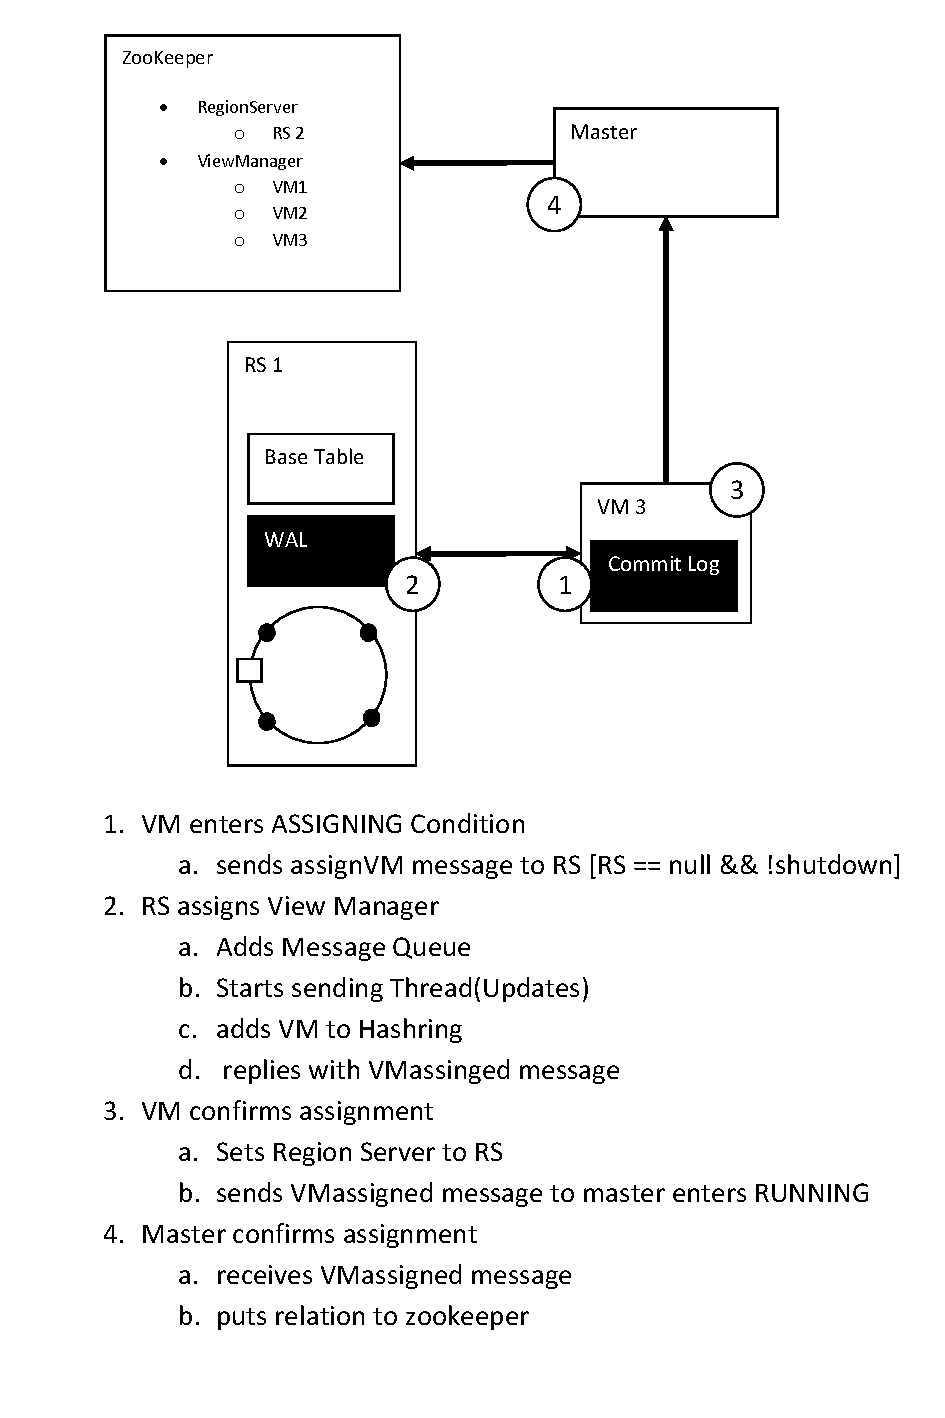
\includegraphics[scale=0.8]{figures/SO_AssignViewManager}
     \caption{Assign View Manager}
    \label{fig:assignviewmanager}
\end{figure}
\newpage

\section{Withdraw View Manager}
\begin{figure}[h!]
  \centering
    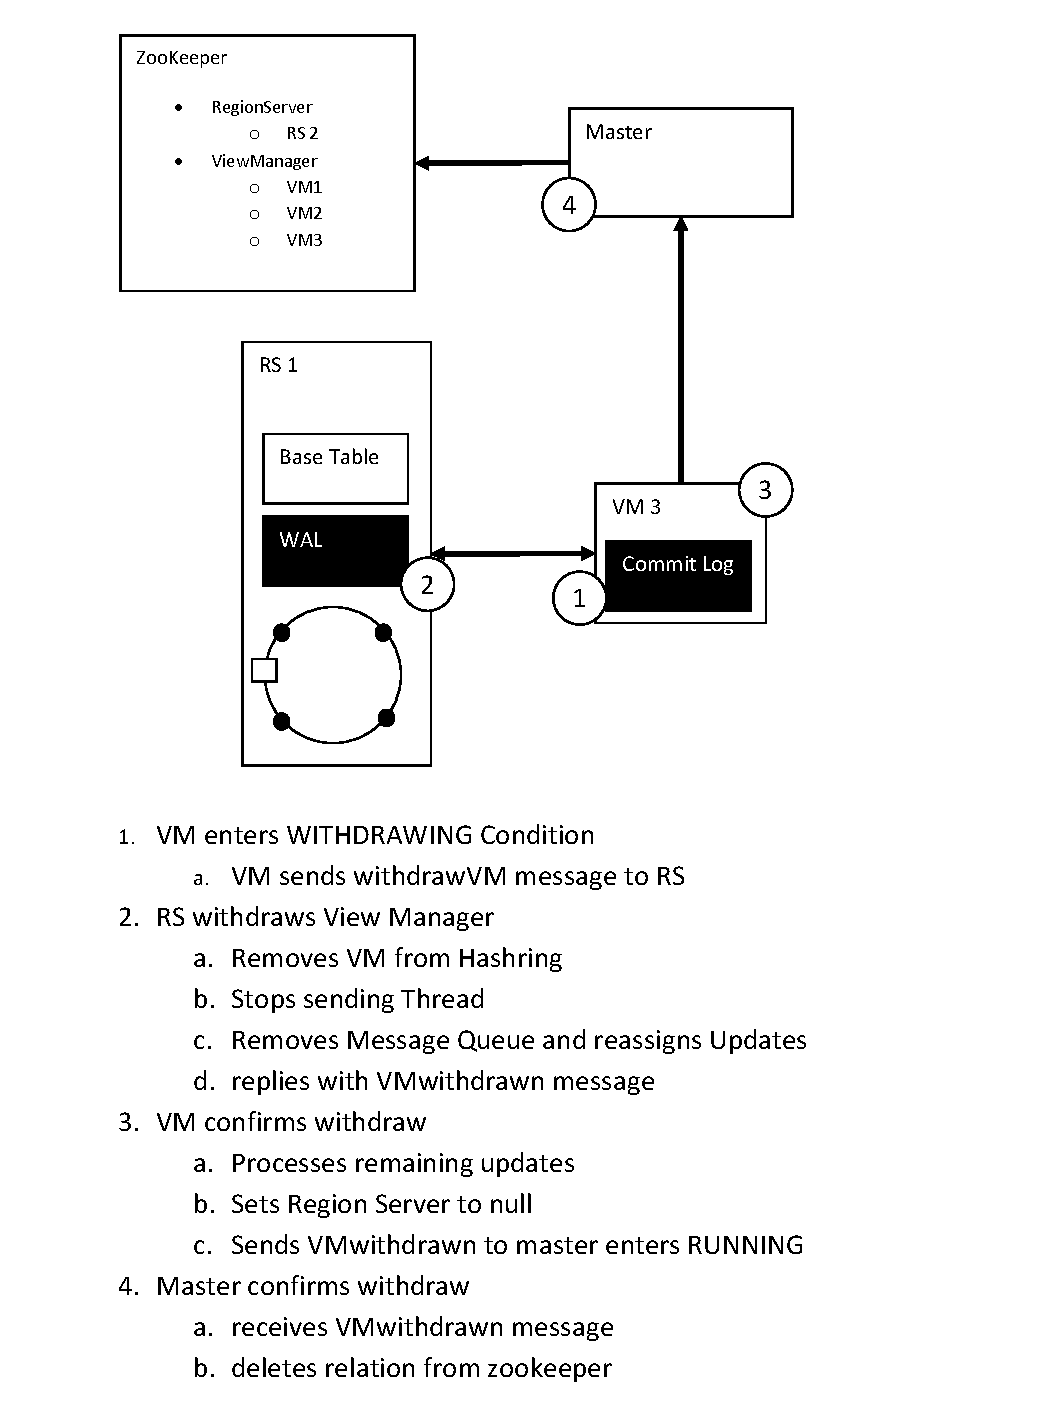
\includegraphics[scale=0.8]{figures/SO_WithdrawViewManager}
     \caption{Withdraw View Manager}
    \label{fig:withdrawviewmanager}
\end{figure}
\newpage
\section{Reassign View Manager}
\begin{figure}[h!]
  \centering
    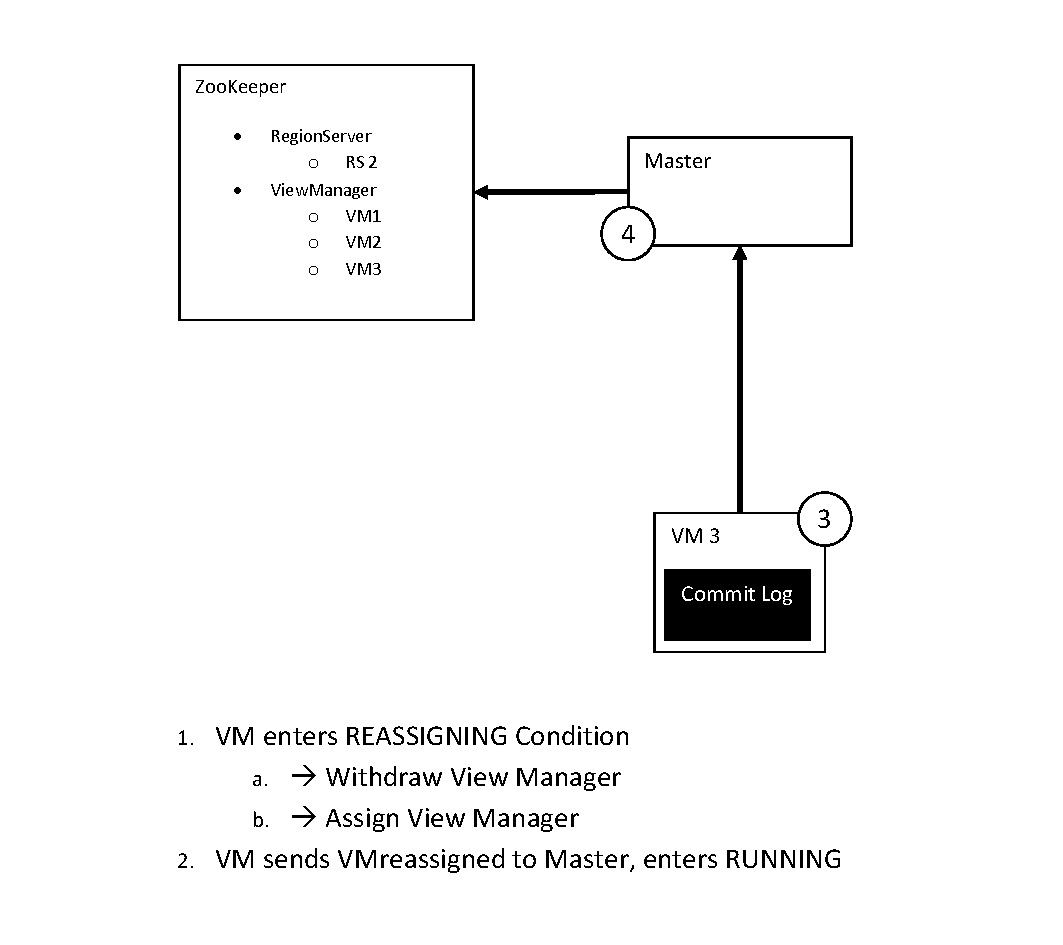
\includegraphics[scale=0.8]{figures/SO_ReassignViewManager}
     \caption{Reassign View Manager}
    \label{fig:reassignviewmanager}
\end{figure}

\newpage

\section{View Manager Crash}
\begin{figure}[h!]
  \centering
    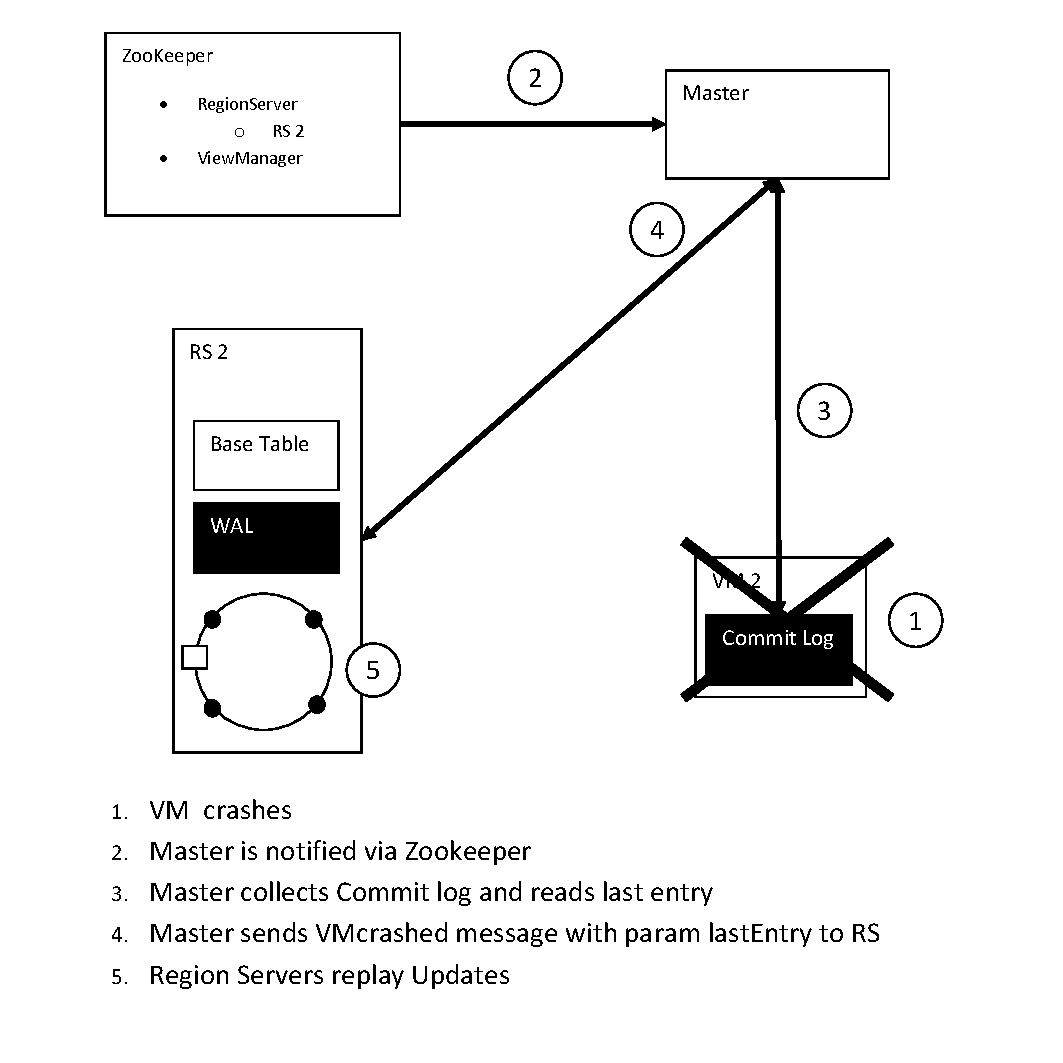
\includegraphics[scale=0.8]{figures/SO_ViewManagerCrash}
     \caption{View Manager Crash}
    \label{fig:so_viewmanagercrash}
\end{figure}
\newpage

\section{Add Region Server}
\begin{figure}[h!]
  \centering
    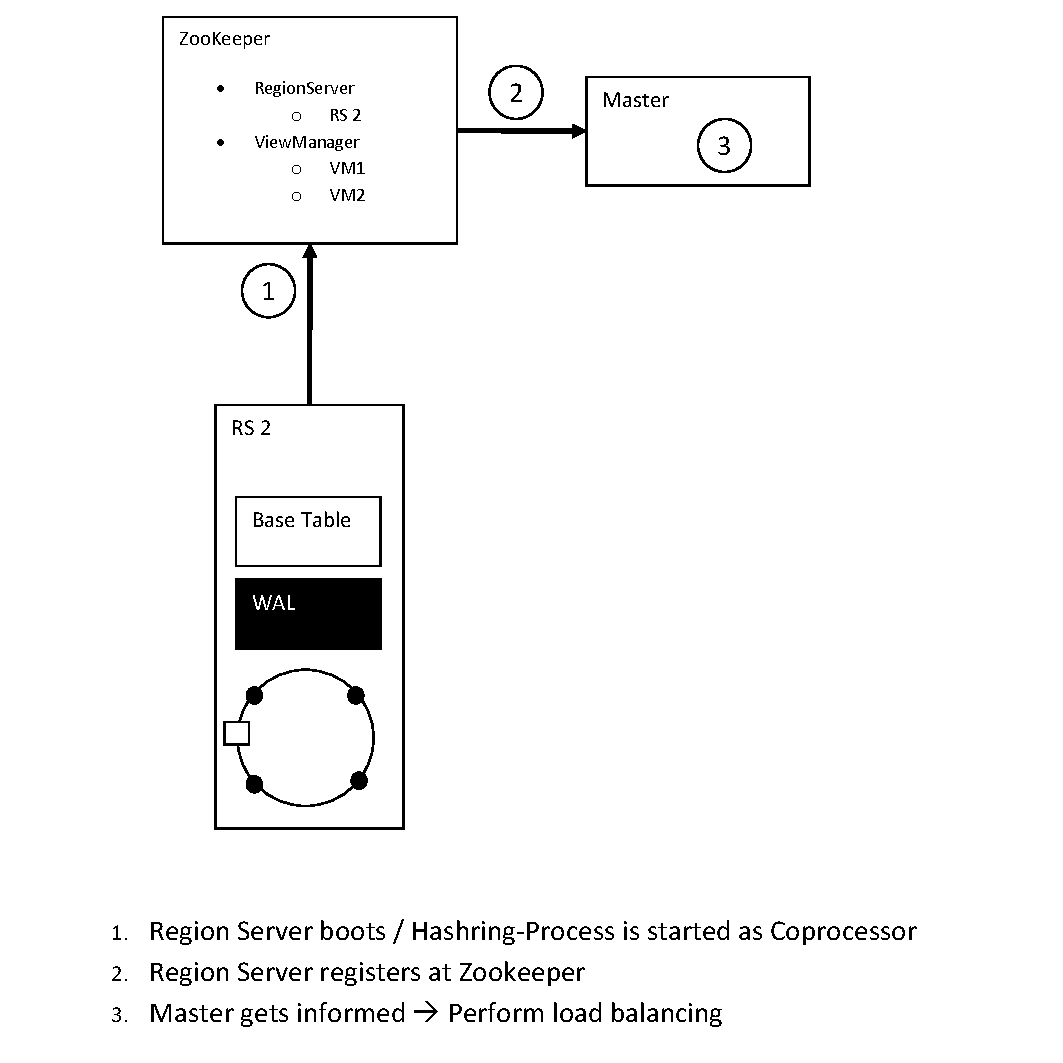
\includegraphics[scale=0.8]{figures/SO_AddRegionServer}
     \caption{Add Region Server}
    \label{fig:addregionserver}
\end{figure}
\newpage

\section{Region Server Crash}
\begin{figure}[h!]
  \centering
    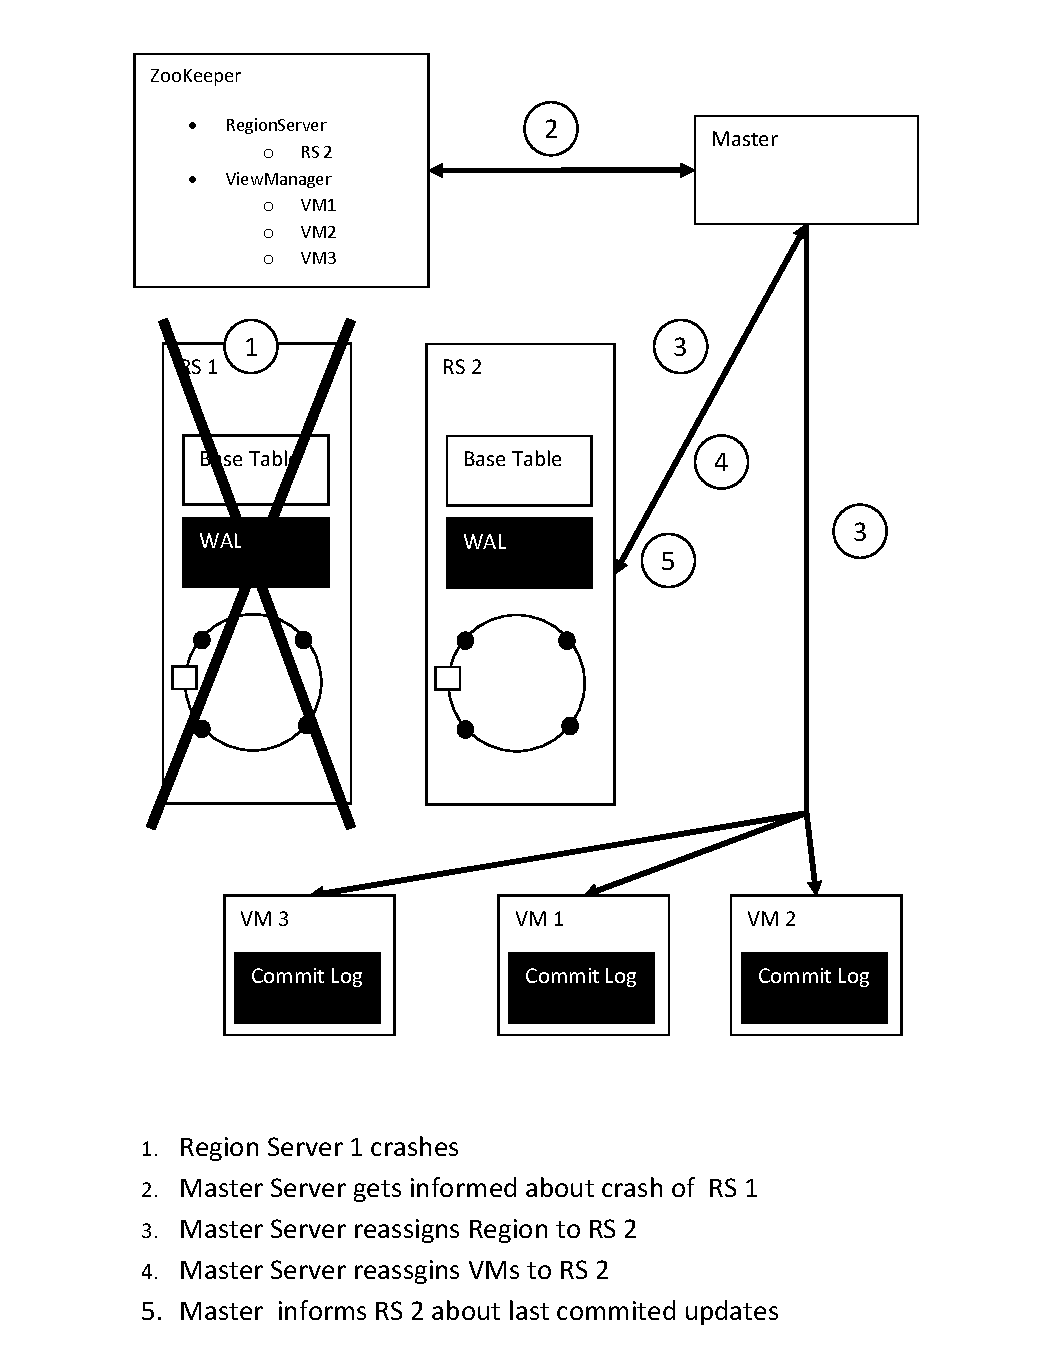
\includegraphics[scale=0.8]{figures/SO_RegionServerCrash}
     \caption{Region Server Crash}
    \label{fig:regionservercrash}
\end{figure}
\newpage

\section{Update Processing}
\begin{figure}[h!]
  
  \centering
    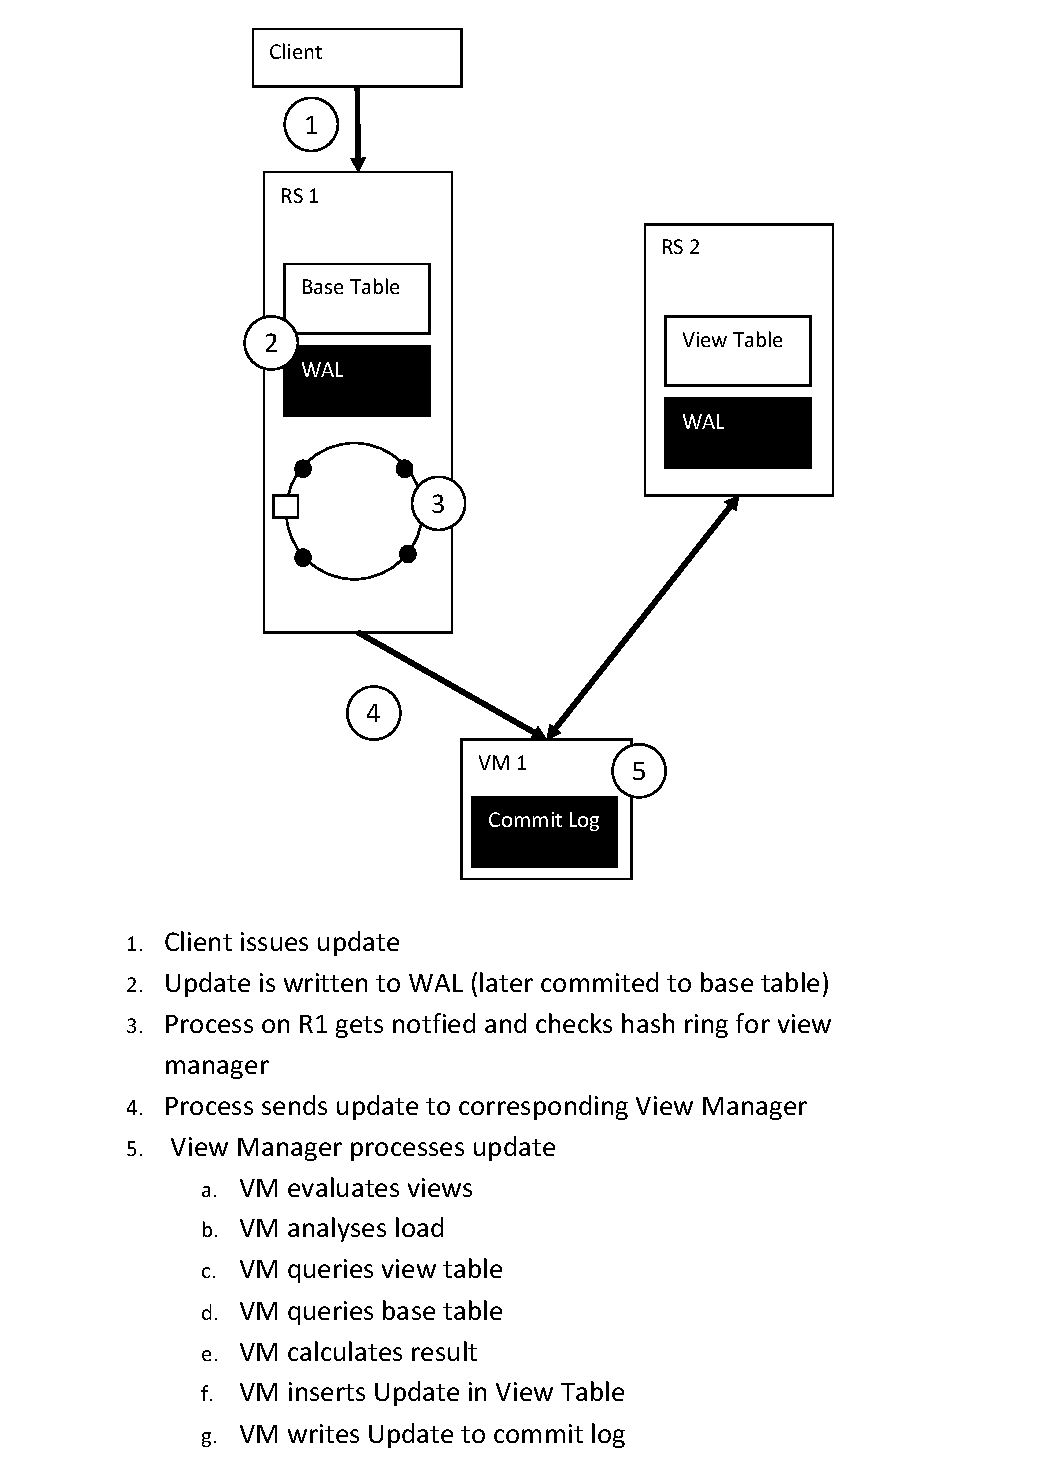
\includegraphics[scale=0.7]{figures/SO_UpdateProcessing}
    \caption{Update Path}
    \label{fig:updatepath}
\end{figure}

\newpage
\section{Status Reports}
\begin{figure}[h!]
  
  \centering
    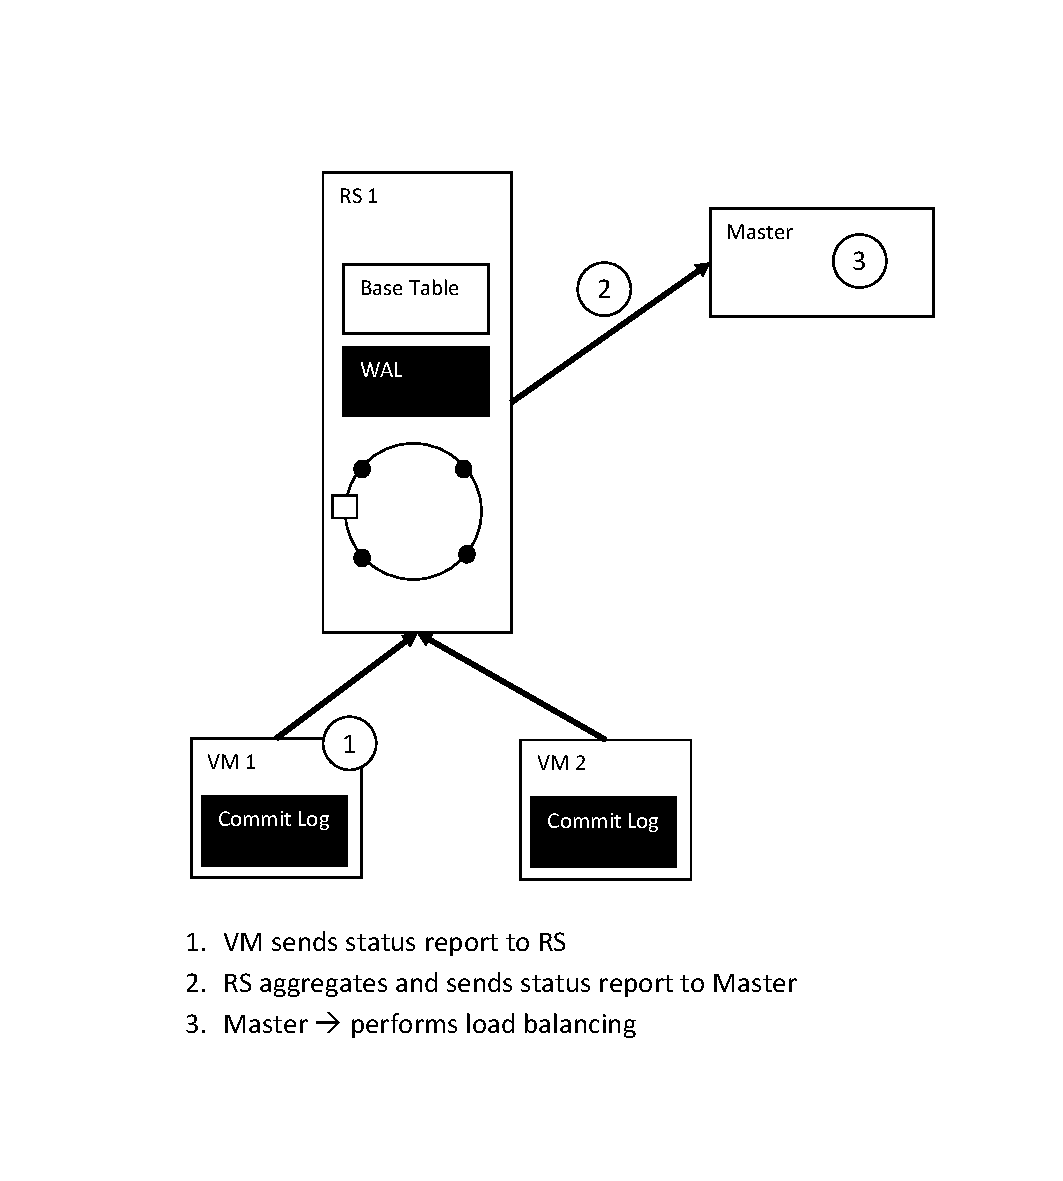
\includegraphics[width=\linewidth]{figures/SO_StatusReports}
    \caption{Status Reports}
    \label{fig:statusreports}
\end{figure}

\chapter{View Consistency}
\label{chapter:viewconsistencyappendix}


\section{Challenges to consistency}
\begin{figure}[h!]
  \centering
    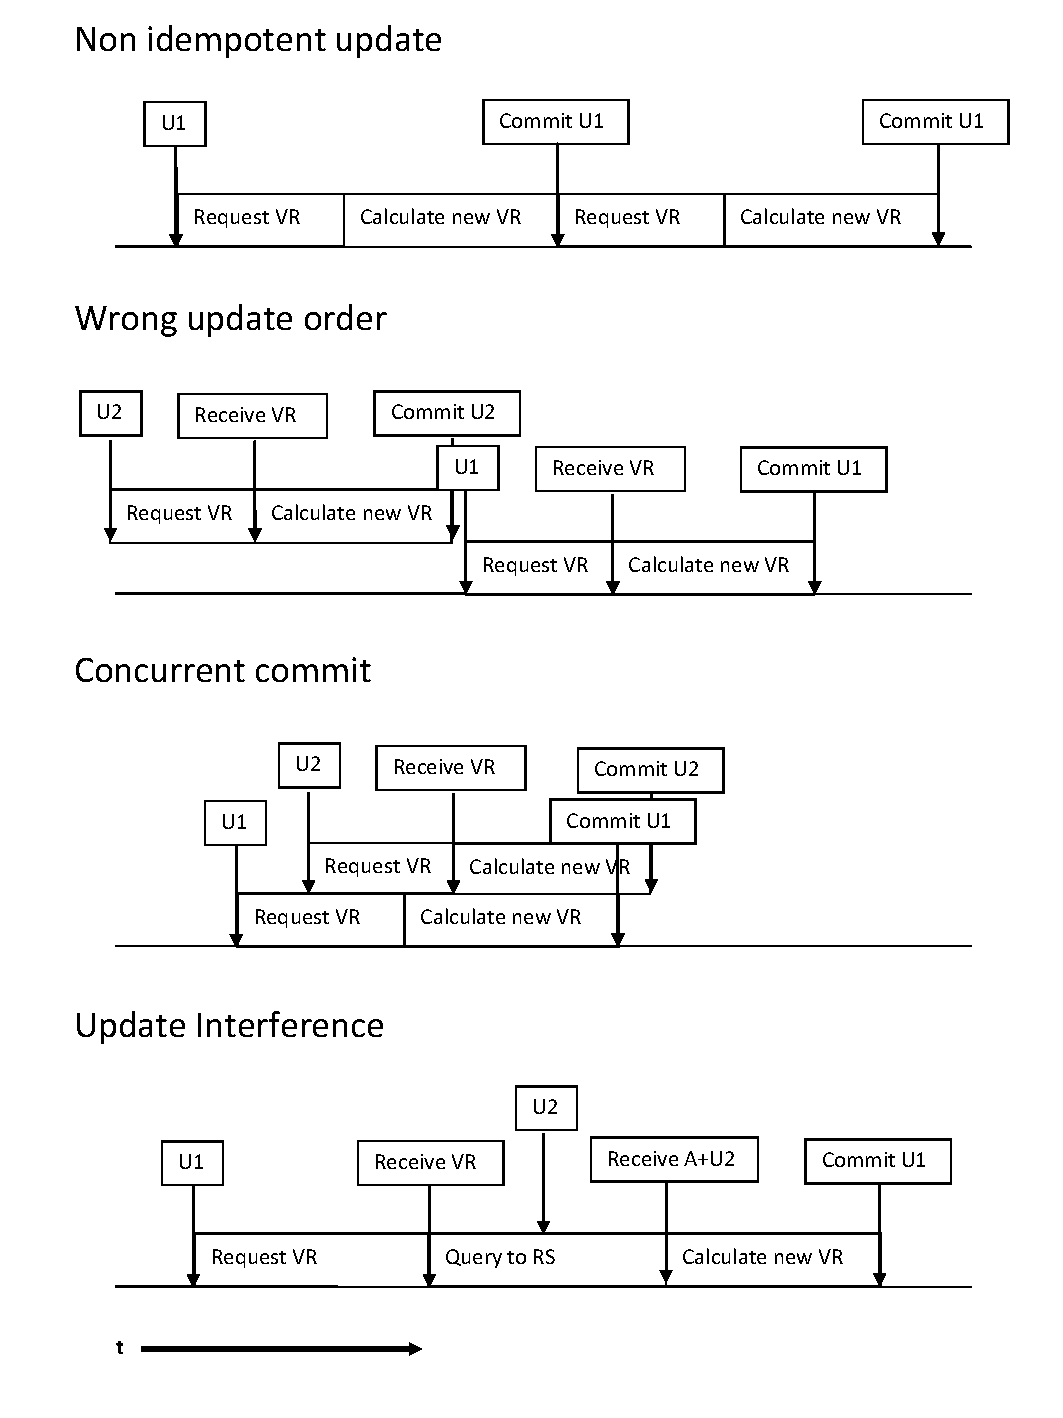
\includegraphics[scale=0.6]{figures/CO_ConsistencyProblems}
     \caption{Consistency threats}
    \label{fig:co_consistencyproblems}
\end{figure}
\newpage

\subsection{Non idempotent view updates}
\begin{figure}[h!]
  \centering
    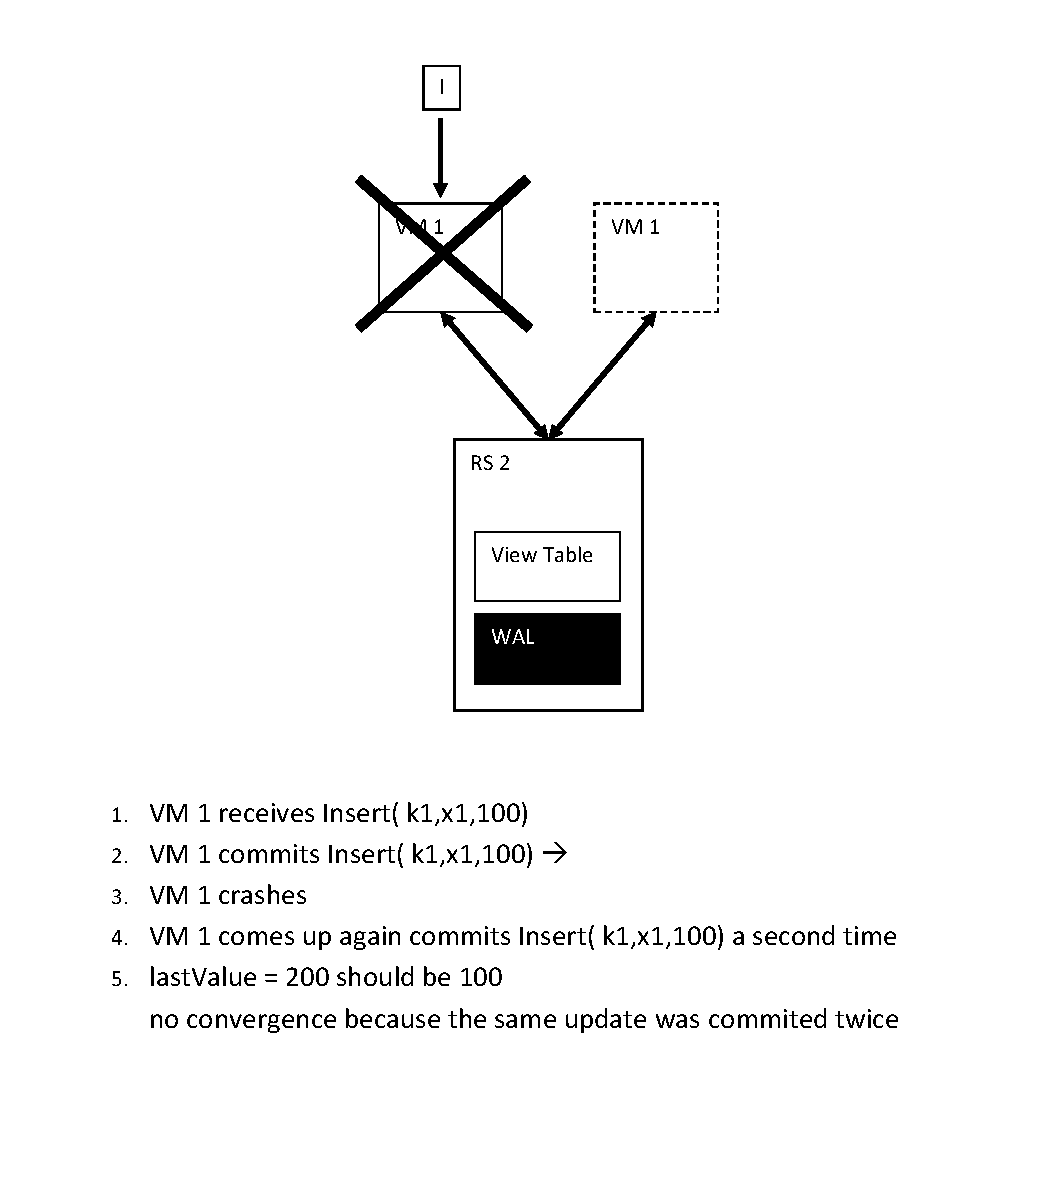
\includegraphics[scale=0.8]{figures/CO_NonIdempotentViewUpdates}
     \caption{Non idempotent view update}
    \label{fig:co_nonidempotentviewupdates}
\end{figure}

\newpage

\subsection{Wrong update order}
\begin{figure}[h!]
  \centering
    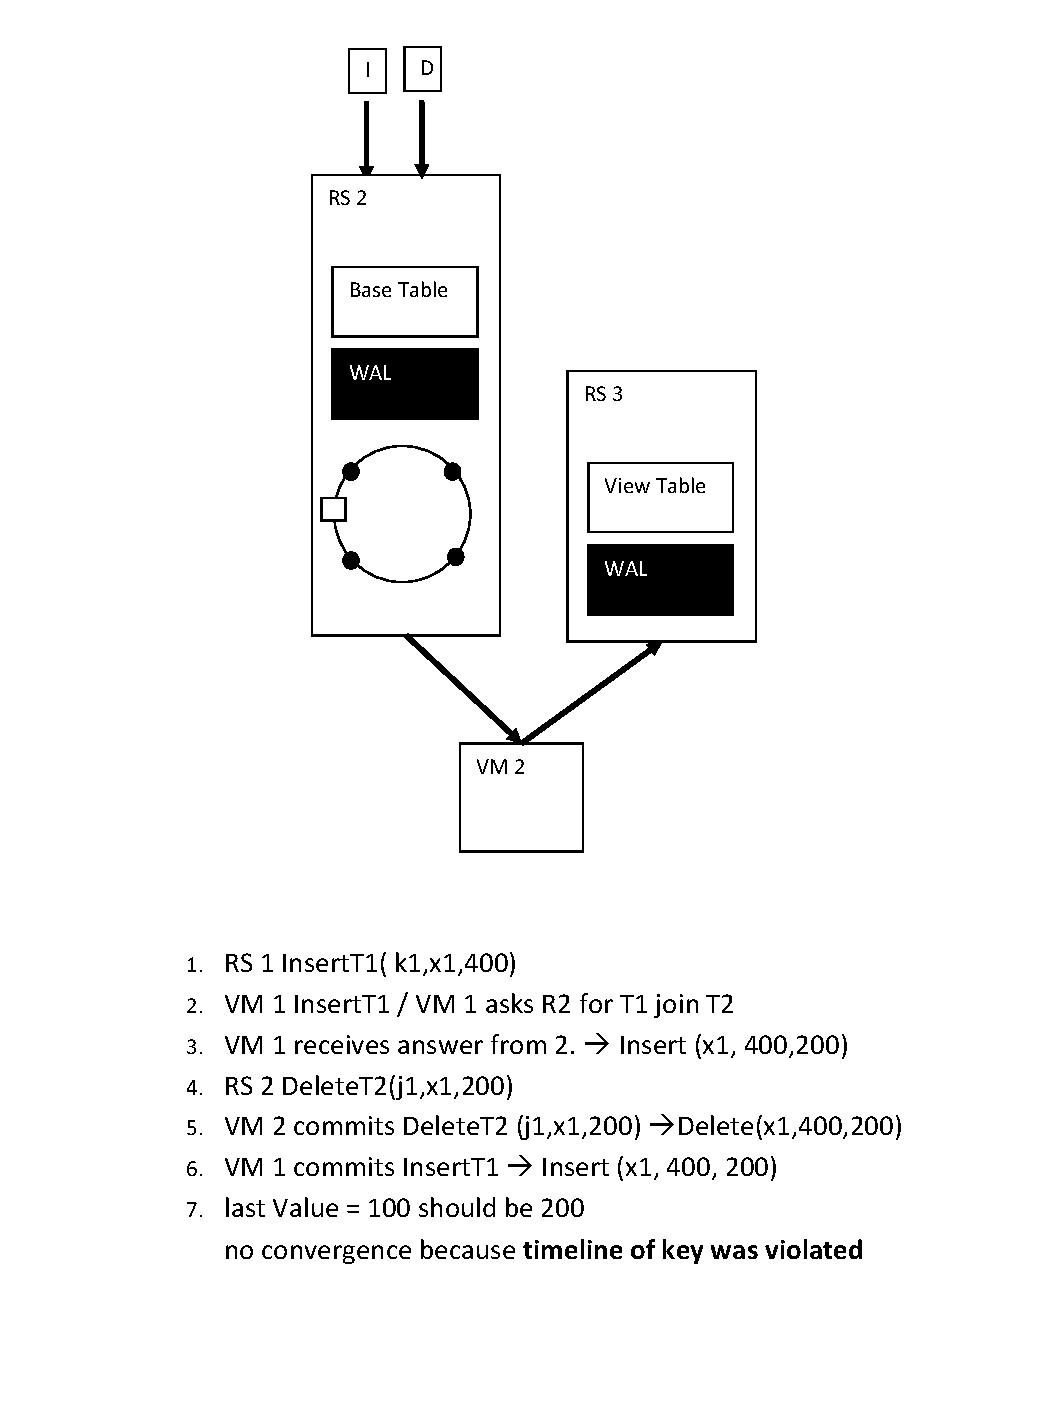
\includegraphics[scale=0.8]{figures/CO_WrongUpdateOrderJoin}
     \caption{Wrong update order join}
    \label{fig:co_wrongupdateorderjoin}
\end{figure}
\newpage
\begin{figure}[h!]
  \centering
    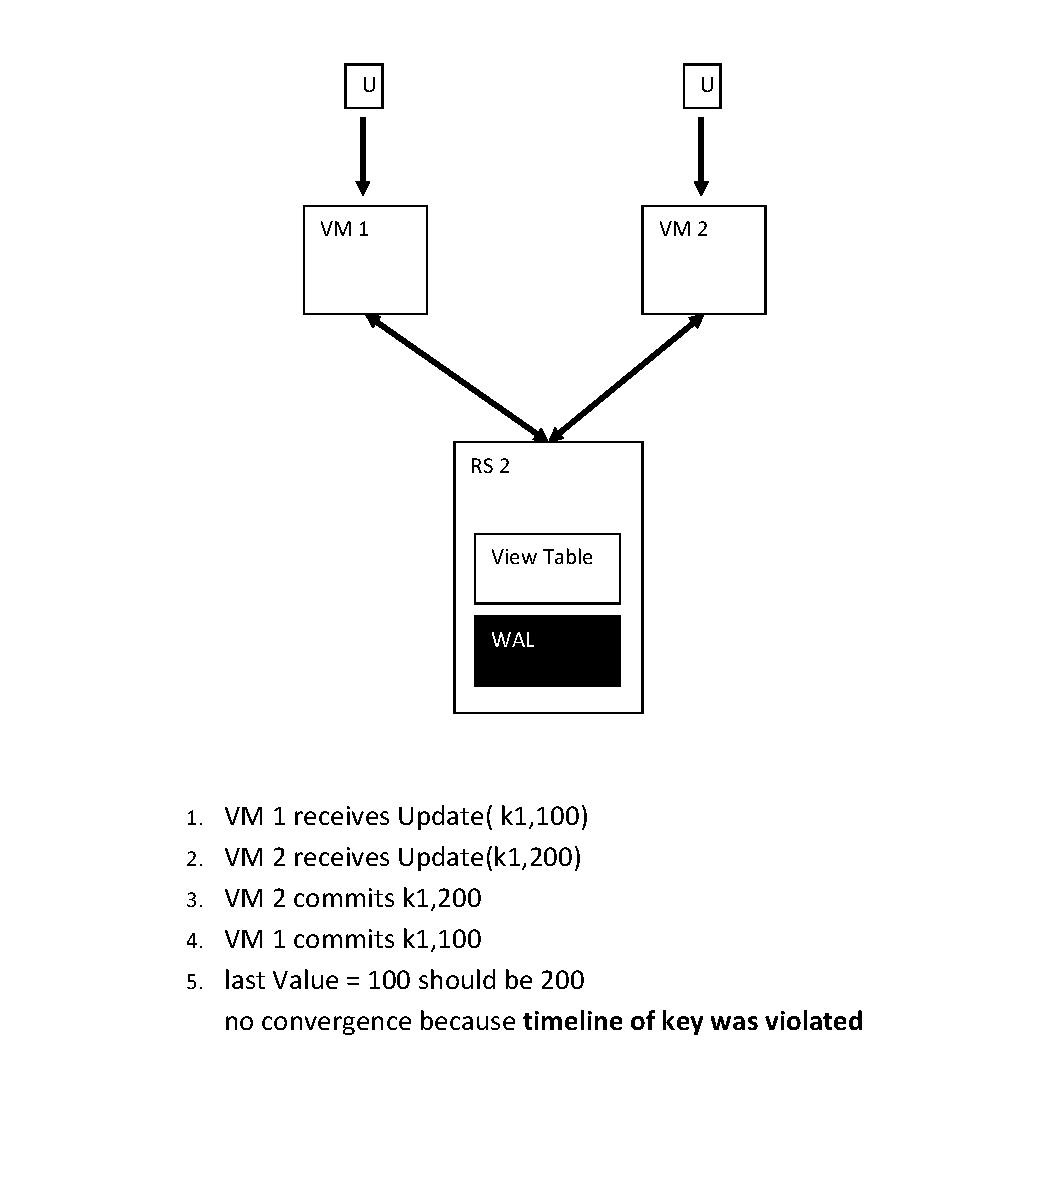
\includegraphics[scale=0.8]{figures/CO_WrongUpdateOrderSelection}
     \caption{Wrong update order Selection}
    \label{fig:co_wrongupdateorderselection}
\end{figure}
\newpage

\subsection{Concurrent commit}
\begin{figure}[h!]
  \centering
    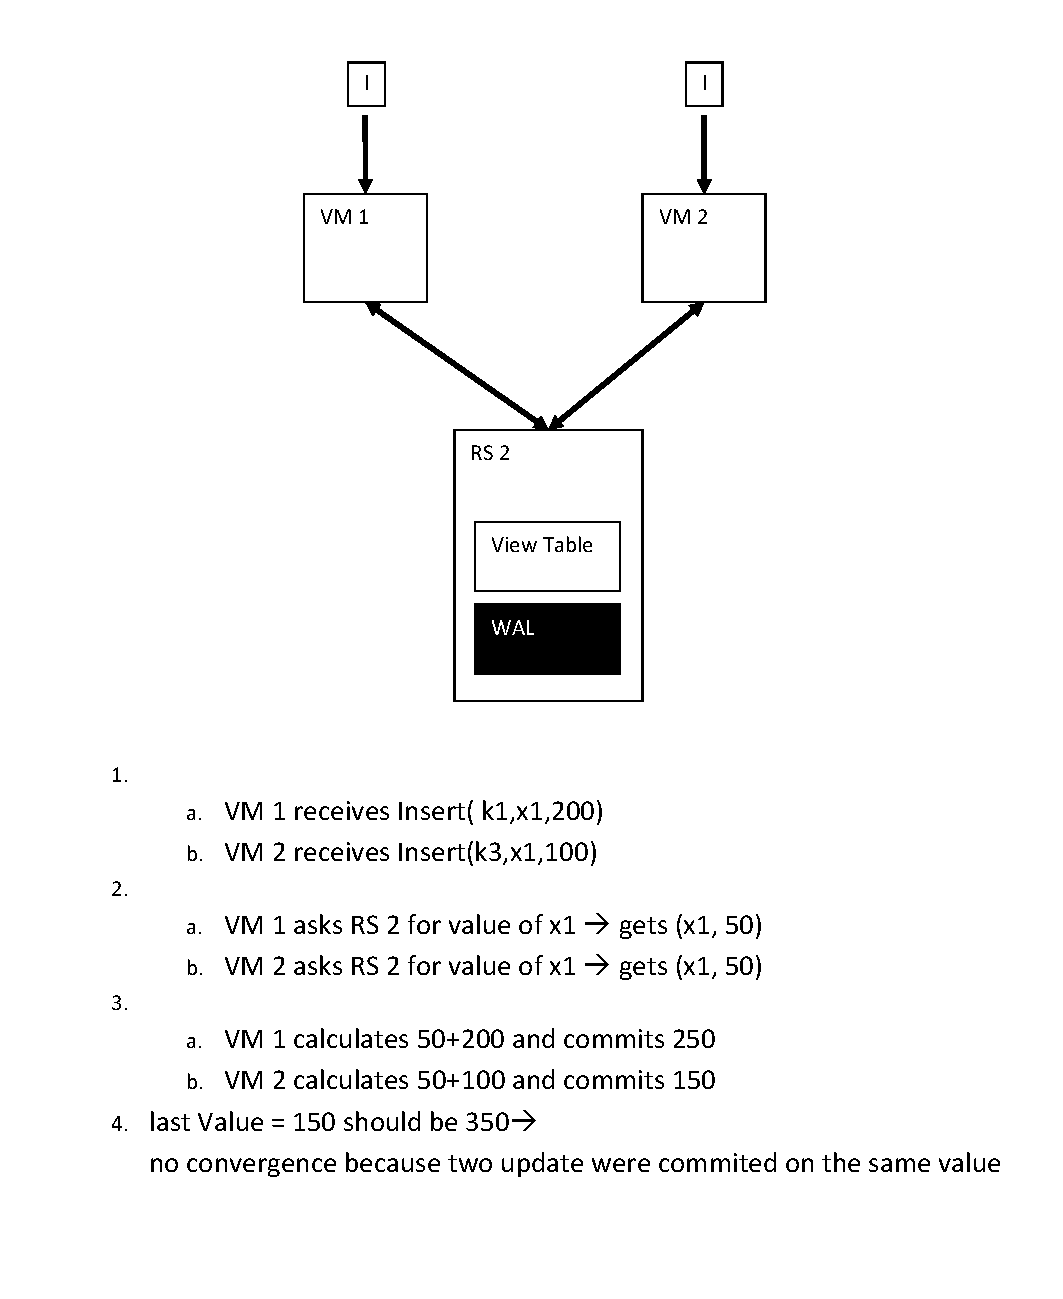
\includegraphics[scale=0.8]{figures/CO_ConcurrentCommitSum}
     \caption{Concurrent commit sum}
    \label{fig:co_concurrentcommitsum}
\end{figure}
\newpage
\begin{figure}[h!]
  \centering
    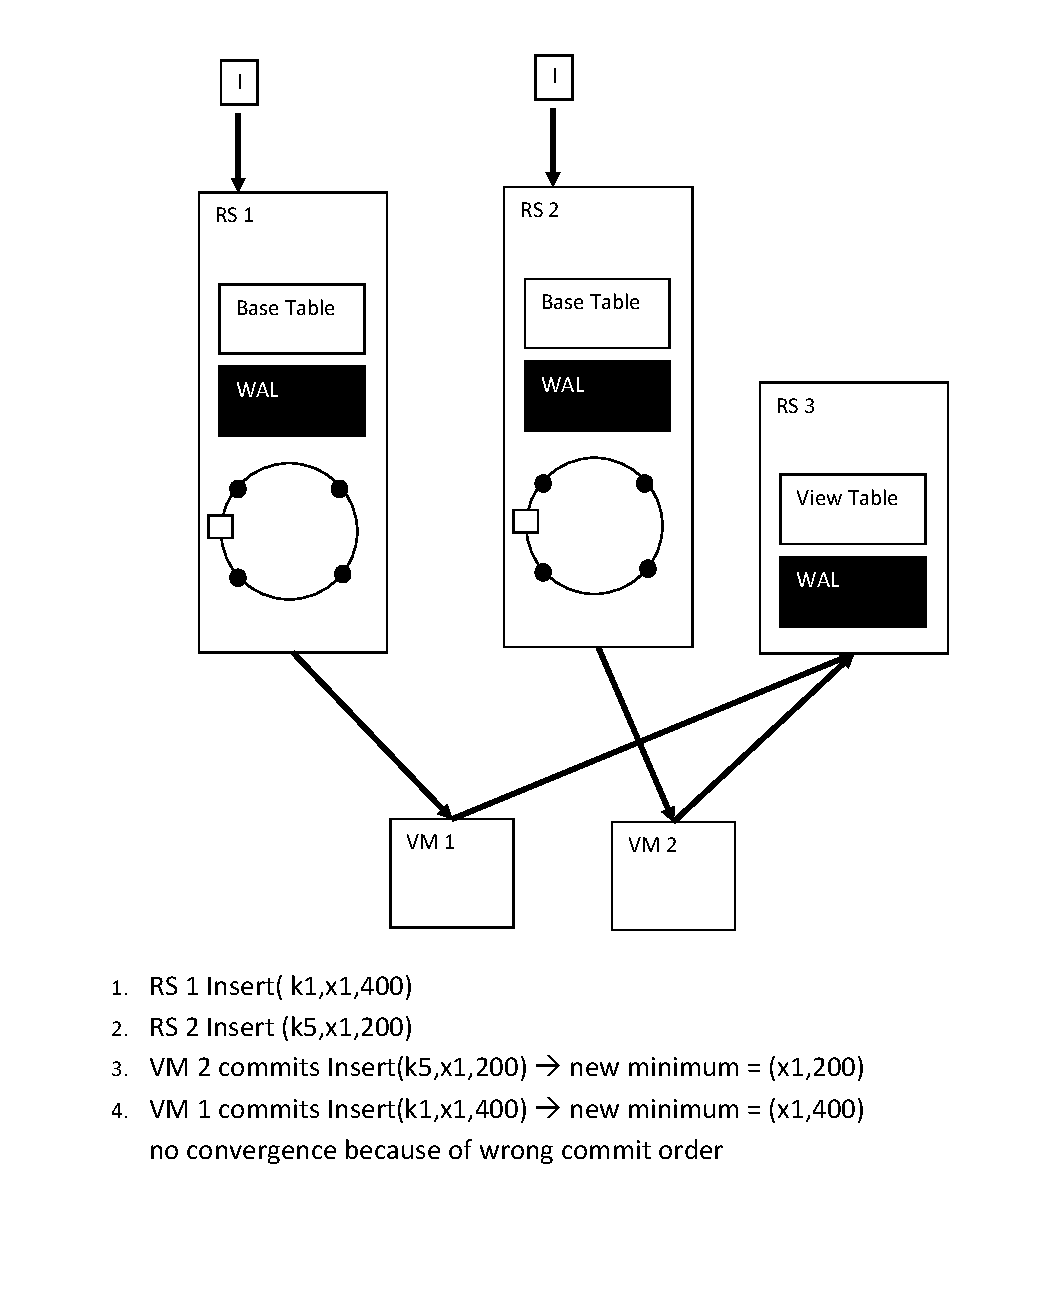
\includegraphics[scale=0.8]{figures/CO_ConcurrentCommitMin}
     \caption{Concurrent commit min}
    \label{fig:co_concurrentcommitmin}
\end{figure}
\newpage

\subsection{Update interference}
\begin{figure}[h!]
  \centering
    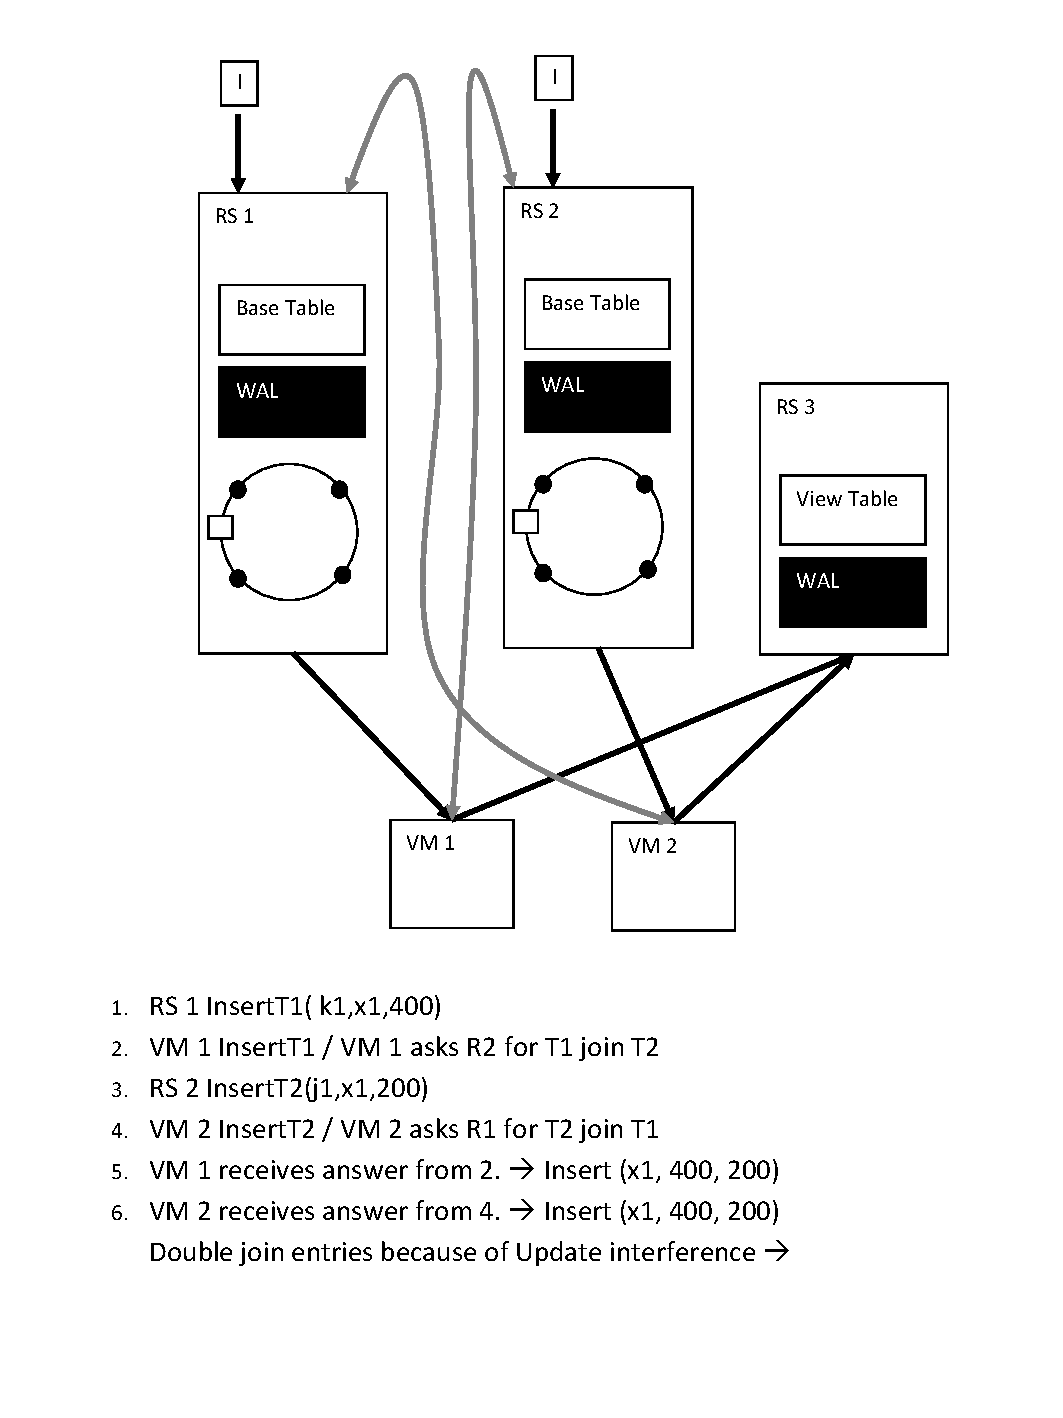
\includegraphics[scale=0.8]{figures/CO_UpdateInterferenceJoin}
     \caption{Update interference join}
    \label{fig:co_updateinterferencejoin}
\end{figure}
\newpage
\begin{figure}[h!]
  \centering
    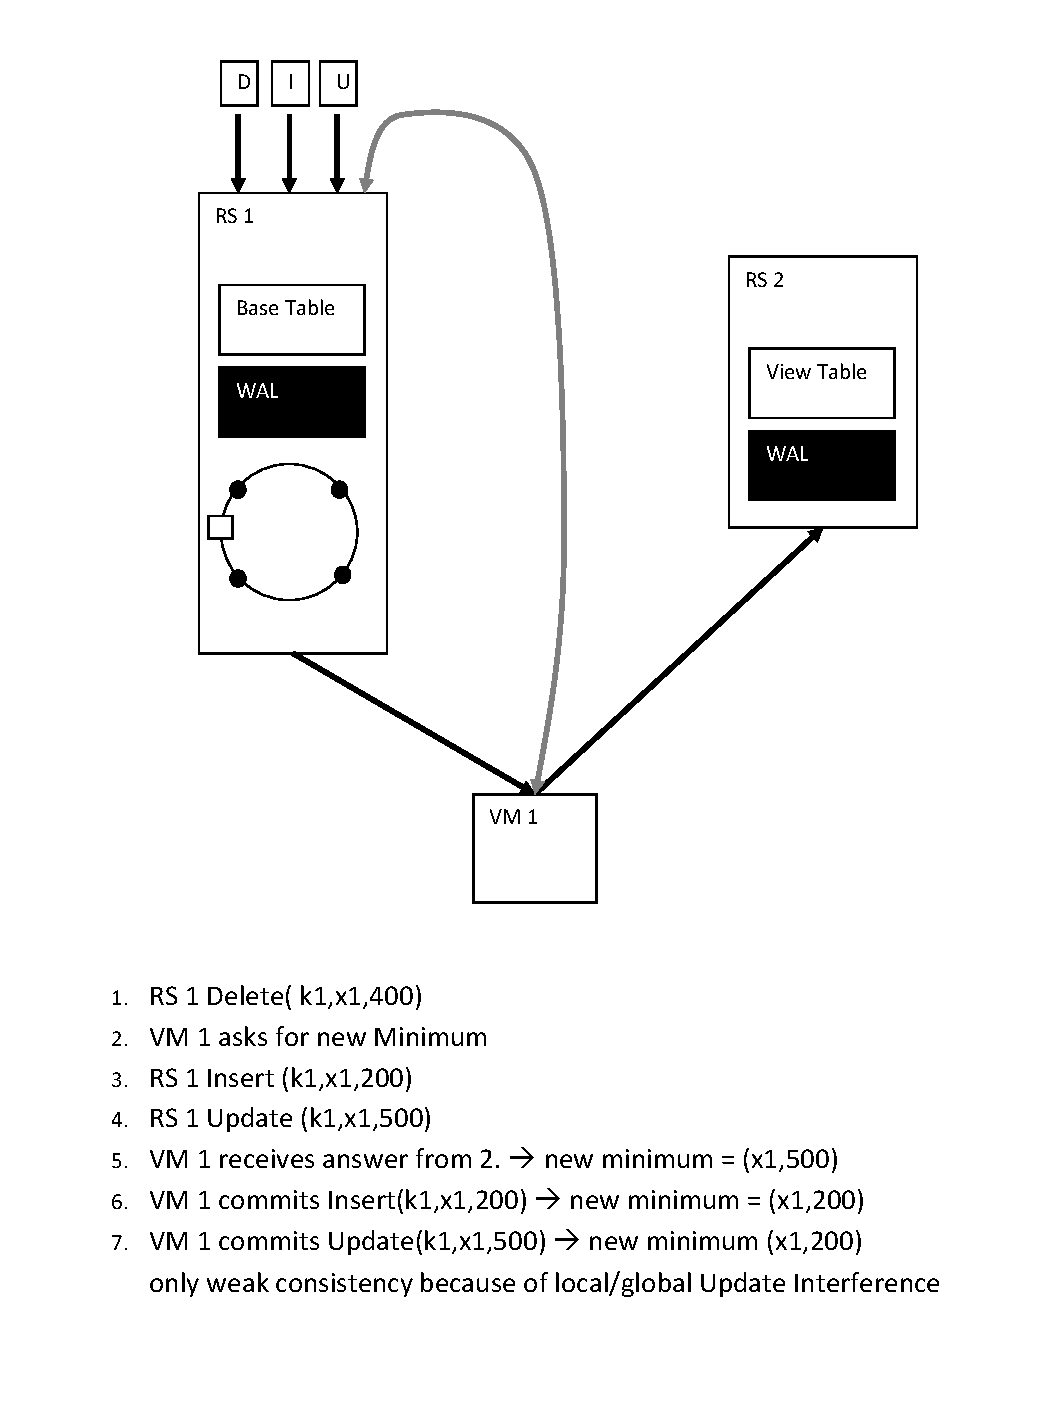
\includegraphics[scale=0.8]{figures/CO_UpdateInterferenceMin}
     \caption{Update interference min}
    \label{fig:co_updateinterferencemin}
\end{figure}
\newpage

\chapter{Load Balancing}
\label{chapter:loadbalancingappendix}


\section{Add View Manager}
\begin{figure}[h!]
  \centering
    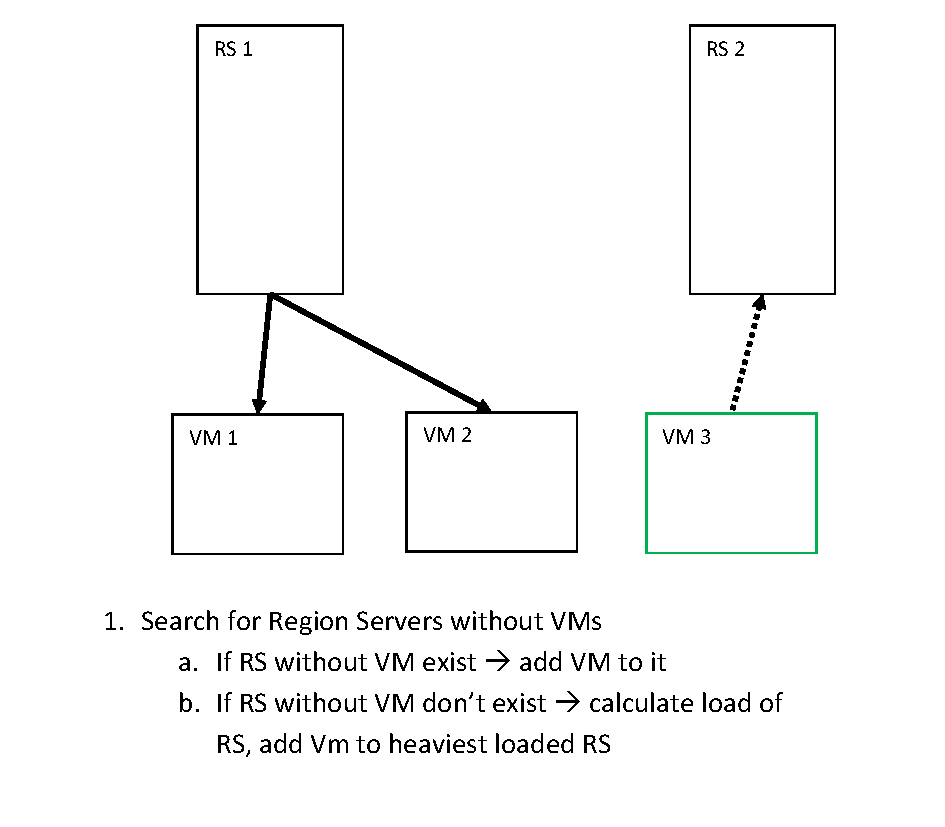
\includegraphics[scale=0.8]{figures/LB_AddViewManager}
     \caption{Add View Manager}
    \label{fig:lb_addviewmanager}
\end{figure}
\newpage

\section{Remove View Manager}
\begin{figure}[h!]
  \centering
    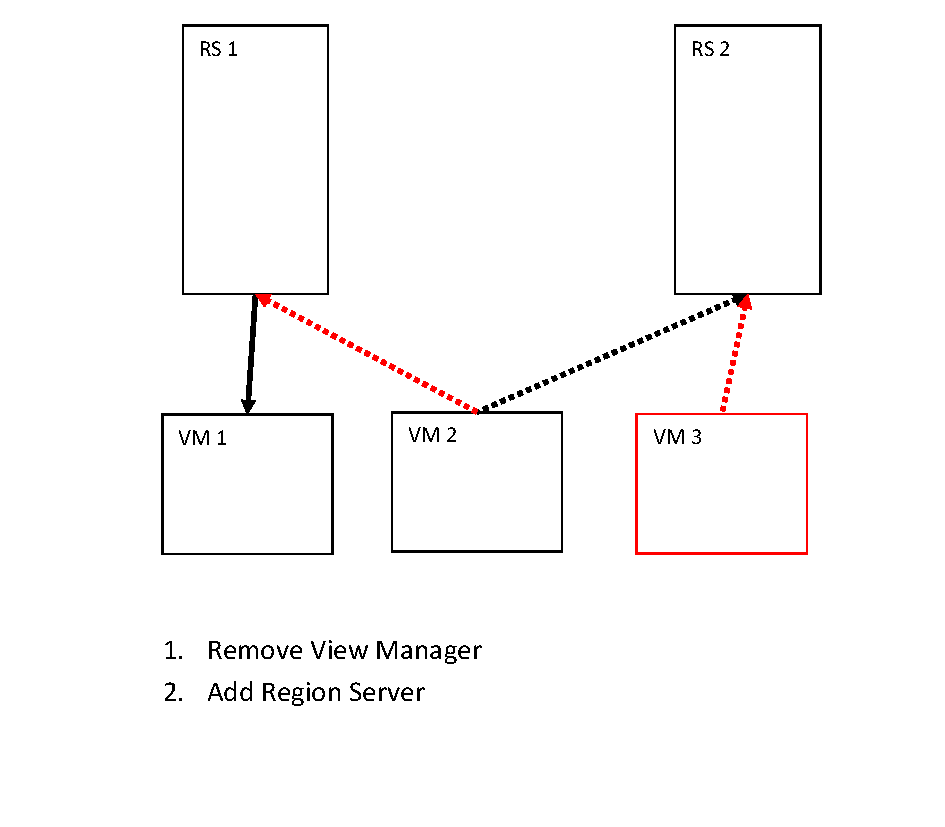
\includegraphics[scale=0.8]{figures/LB_RemoveViewManager}
     \caption{Remove View Manager}
    \label{fig:lb_removeviewmanager}
\end{figure}
\newpage

\section{Add Region Server}
\begin{figure}[h!]
  \centering
    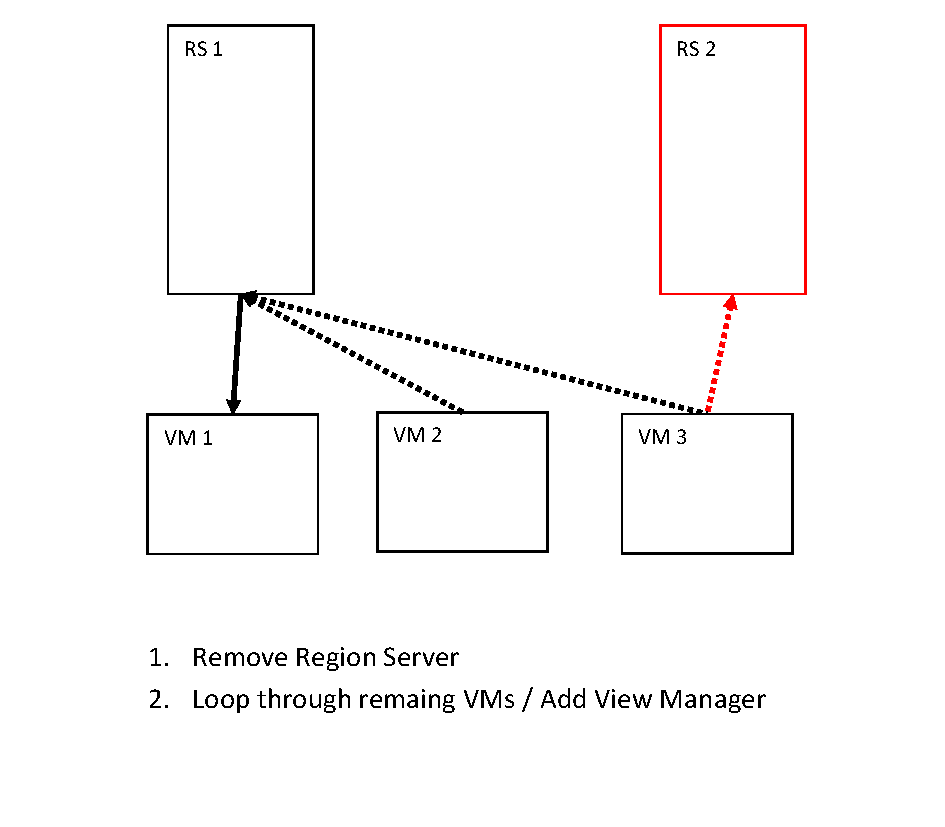
\includegraphics[scale=0.8]{figures/LB_AddRegionServer}
     \caption{Add Region Server}
    \label{fig:lb_addregionserver}
\end{figure}
\newpage

\section{Remove Region Server}
\begin{figure}[h!]
  \centering
    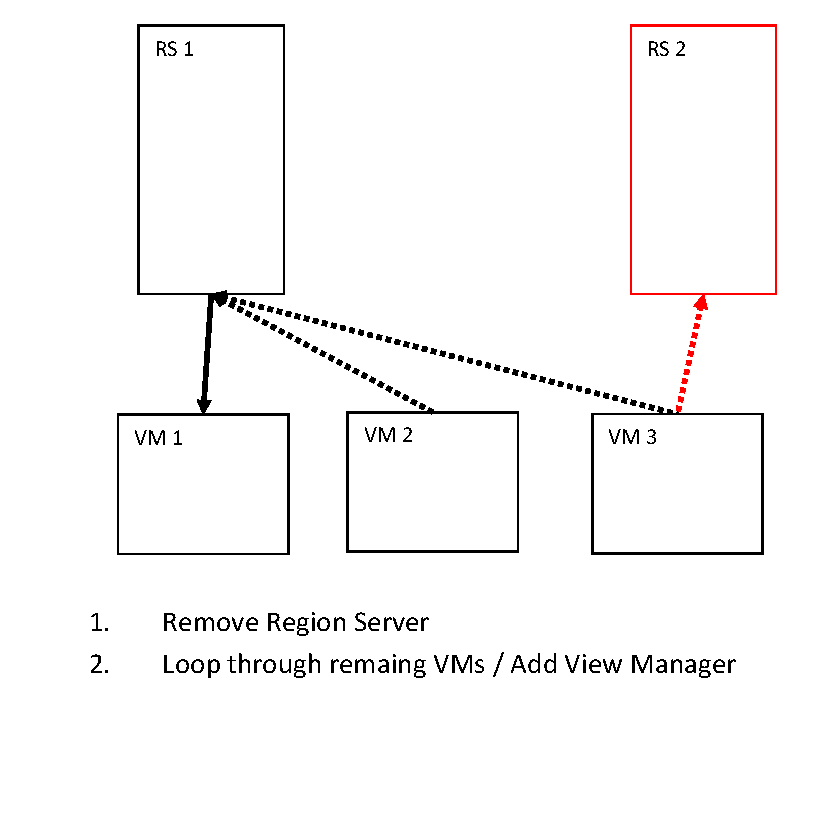
\includegraphics[scale=0.8]{figures/LB_RemoveRegionServer}
    \caption{Remove Region Server}
    \label{fig:lb_removeregionserver}
\end{figure}
\newpage




  \clearemptydoublepage
  
	\bibliography{bibliography/literature}
	
 
\end{document}

